%%%%%%%%%%%%%%%%%%%%%%%%%%%%%%%%%%%%%%%%%
% Beamer Presentation
% LaTeX Template
% Version 1.0 (10/11/12)
%
% This template has been downloaded from:
%----------------------------------------------------------------------------------------

\documentclass[aspectratio=169]{beamer}
%%\documentclass{beamer}
\usetheme{Madrid}
\usepackage{todonotes}
\usepackage{graphicx}
\usepackage{xcolor}
\usepackage{subfig}
%%\usepackage[noend]{algpseudocode}


\usepackage{algorithm}
\usepackage{algorithmic}

\usepackage{blkarray}
\usepackage{amsmath}
\usepackage{xspace}
\usepackage{float}
%\usepackage{enumitem}




\usepackage{tikz}
\usetikzlibrary{matrix, decorations, patterns, positioning, shapes, 3d,calc, intersections, arrows, fit, hobby}
%%\usetikzlibrary{matrix, decorations, patterns, positioning, shapes, 3d, calc, intersections, arrows, fit}
%%\usepackage{enumitem}

\mode<presentation> {

% The Beamer class comes with a number of default slide themes
% which change the colors and layouts of slides. Below this is a list
% of all the themes, uncomment each in turn to see what they look like.

%\usetheme{default}
%\usetheme{AnnArbor}
%\usetheme{Antibes}
%\usetheme{Bergen}
%\usetheme{Berkeley}
%\usetheme{Berlin}
%\usetheme{Boadilla}
%\usetheme{CambridgeUS}
%\usetheme{Copenhagen}
%\usetheme{Darmstadt}
%\usetheme{Dresden}
%\usetheme{Frankfurt}
%\usetheme{Goettingen}
%\usetheme{Hannover}
%\usetheme{Ilmenau}
%\usetheme{JuanLesPins}
%\usetheme{Luebeck}
\usetheme{Madrid}
%\usetheme{Malmoe}
%\usetheme{Marburg}
%\usetheme{Montpellier}
%\usetheme{PaloAlto}
%\usetheme{Pittsburgh}
%\usetheme{Rochester}
%\usetheme{Singapore}
%\usetheme{Szeged}
%\usetheme{Warsaw}

% As well as themes, the Beamer class has a number of color themes
% for any slide theme. Uncomment each of these in turn to see how it
% changes the colors of your current slide theme.

%\usecolortheme{albatross}
%\usecolortheme{beaver}
%\usecolortheme{beetle}
%\usecolortheme{crane}
%\usecolortheme{dolphin}
%\usecolortheme{dove}
%\usecolortheme{fly}
%\usecolortheme{lily}
%\usecolortheme{orchid}
%\usecolortheme{rose}
%\usecolortheme{seagull}
%\usecolortheme{seahorse}
%\usecolortheme{whale}
%\usecolortheme{wolverine}

%\setbeamertemplate{footline} % To remove the footer line in all slides uncomment this line
%\setbeamertemplate{footline}[page number] % To replace the footer line in all slides with a simple slide count uncomment this line

%\setbeamertemplate{navigation symbols}{} % To remove the navigation symbols from the bottom of all slides uncomment this line
}


\usepackage{booktabs} % Allows the use of \toprule, \midrule and \bottomrule in tables



\newcommand{\lowerbound}{{\sc C_{LB}}\xspace}
\newcommand{\maxp}{{\sc MaxP}\xspace}
\newcommand{\lowerboundmatrix}{{\sc LB(MatrixComm)}\xspace}
\newcommand{\lowerboundtensor}{{\sc LB(TensorComm)}\xspace}
\newcommand{\odata}{{\sc O_d}\xspace}
\newcommand{\init}[1]{\hat{#1}}
\newcommand{\tmp}[1]{q_{prev}}
\newcommand{\lbbasedpartition}{{\it Algo1($C_{LB}$ based config)}\xspace}
\newcommand{\bestconfigAAO}{{\it Algo1(best config)}\xspace}
\newcommand{\bestconfigSeq}{{\it Seq-Appr(best config)}\xspace}

\newcommand{\A}{\mathbf{A}}
\newcommand{\B}{\mathbf{B}}
\newcommand{\CC}{\mathbf{C}}


\newcommand{\tensorcolor}{cyan}

%% Colors from https://latexcolor.com/
\definecolor{pastelviolet}{rgb}{0.8, 0.6, 0.79}
\definecolor{babyblueeyes}{rgb}{0.63, 0.79, 0.95}
\definecolor{pastelyellow}{rgb}{0.99, 0.99, 0.59}
\definecolor{pastelgreen}{rgb}{0.47, 0.87, 0.47}
\definecolor{pastelred}{rgb}{1.0, 0.41, 0.38}
\colorlet{patternblue}{blue!60}


%%For tensor notations
\input{./tensor_header}
\newcommand{\X}{\T{X}}
\newcommand{\Y}{\T{Y}}
\newcommand{\starontop}[1]{{#1}^*}


\graphicspath{{./diagrams/}{./Figs/}{./plots/}}


%%\newcommand{\tensor}[1]{{\cal\textbf{#1}\xspace}}
\newcommand{\tensor}[1]{\T{#1}}



\definecolor{pastelviolet}{rgb}{0.8, 0.6, 0.79}
\definecolor{babyblueeyes}{rgb}{0.63, 0.79, 0.95}
\definecolor{pastelyellow}{rgb}{0.99, 0.99, 0.59}
%%\definecolor{pastelgreen}{rgb}{0.47, 0.87, 0.47}
\definecolor{pastelgreen}{rgb}{0, 1, 0}
\definecolor{pastelred}{rgb}{1.0, 0.41, 0.38}
\colorlet{patternblue}{blue!60}




\definecolor{forestgreen}{rgb}{0.13, 0.55, 0.13}
\definecolor{greenhtml}{rgb}{0.0, 0.5, 0.0}
\definecolor{cyannew}{rgb}{0.0, 1.0, 1.0}


\newcommand{\mycolora}{green}
\newcommand{\mycolorb}{blue}
\newcommand{\mycolorc}{cyan}
\newcommand{\mycolord}{violet}
\newcommand{\mycolore}{orange}
\newcommand{\mycolorf}{forestgreen}


%%\newcommand{\mysymbola}{\textcolor{\mycolora}{$\blacksquare$}}
%%\newcommand{\mysymbolb}{\textcolor{\mycolorb}{$\blacksquare$}}
%%\newcommand{\mysymbolc}{\textcolor{\mycolorc}{$\blacksquare$}}
%%\newcommand{\mysymbold}{\textcolor{\mycolord}{$\blacksquare$}}
%%\newcommand{\mysymbole}{\textcolor{\mycolore}{$\blacksquare$}}
%%\newcommand{\mysymbolf}{\textcolor{\mycolorf}{$\blacksquare$}}
\newcommand{\mysymbola}{\textcolor{\mycolora}{}}
\newcommand{\mysymbolb}{\textcolor{\mycolorb}{}}
\newcommand{\mysymbolc}{\textcolor{\mycolorc}{}}
\newcommand{\mysymbold}{\textcolor{\mycolord}{}}
\newcommand{\mysymbole}{\textcolor{\mycolore}{}}
\newcommand{\mysymbolf}{\textcolor{\mycolorf}{}}


\newcommand{\mybullet}{\textcolor{blue}{$\quad\bullet$}\xspace}

%%\newenvironment{beameritemize}
%%{ \begin{itemize}
%%		\setlength{\itemsep}{1.5ex}
%%		\setlength{\parskip}{0pt}
%%		\setlength{\parsep}{0pt}   
%%		\addtolength{\itemindent}{-2em}  }
%%{ \end{itemize} }


%----------------------------------------------------------------------------------------
%	TITLE PAGE
%----------------------------------------------------------------------------------------

\title[Scalable Tensor Algorithms]{Scalable Tensor Algorithms for Modern Computing Systems} % The short title appears at the bottom of every slide, the full title is only on the title page

\author[Suraj {\sc Kumar}]{Suraj {\sc Kumar}} % Your name


\institute[LIP/LaBRI Applicant]{CNRS LIP/LaBRI Applicant}
%%%%\institute[Inria Paris] % Your institution as it will appear on the bottom of every slide, may be shorthand to save space
%%%%{
%%%%	Alpines team, Inria Paris, France\\ % Your institution for the title page
%%%%	\medskip
%%%%	\textit{Suraj.kumar@inria.fr} % Your email address
%%%%}

%%\date{\today} % Date, can be changed to a custom date

\date{March 3, 2022} % Date, can be changed to a custom date



\makeatletter
\AtBeginPart{%
	\beamer@tocsectionnumber=0\relax
	\setcounter{section}{0}
	%%	\frame{\partpage}%
}
\makeatother

\begin{document}



\begin{frame}
\titlepage % Print the title page as the first slide
\end{frame}


%%
%%\begin{frame}{Resume in timeline}
%%
%%{\small 
%%	%%	Interests: \textcolor{\mycolora}{Tensors}, \textcolor{\mycolorb}{Scalable Algorithms}, \textcolor{\mycolorc}{Scheduling}, \textcolor{\mycolord}{Runtime Systems}, \textcolor{\mycolore}{Performance Optimizations}
%%	%%	\vspace*{-0.125cm}
%%	
%%	\vspace*{0.45cm}
%%	\begin{tikzpicture}[scale=0.6, every node/.style={transform shape}]
%%	
%%	\tikzstyle{taskc}=[circle, thick, draw=black, minimum size=2mm, fill=white]
%%	
%%	%%	\tikzstyle{taskr}=[rectangle, rounded corners, draw=black, minimum size=2mm, fill=none]
%%	\tikzstyle{taskr}=[draw=black, rounded corners, minimum height=8mm, minimum width=8mm, fill=none, text=black]
%%	
%%	\draw [->, ultra thick](-1,0) -- (23.5, 0);
%%	\node (t0) at (0,0) [taskc] {};
%%	\node [above right] at (t0) {Jul 2012};
%%	
%%	\node (t1) at (5,0) [taskc] {};
%%	\node [above right] at (t1) {Dec 2013};
%%	\node (t2) at (10,0) [taskc] {};
%%	\node [above right] at (t2) {Aug 2017};
%%	\node (t3) at (15,0) [taskc] {};
%%	\node [above right] at (t3) {May 2018};
%%	\node (t4) at (20,0) [taskc] {};
%%	\node [above right] at (t4) {Nov 2019};
%%	
%%	
%%	\node (ibmnode) at (2.5, -3) [taskr, align=left] {\textbf{IBM Research, New Delhi, India}\\{\footnotesize Software Engineer}};
%%	\node [below, align=left, anchor=north west] at (ibmnode.south west) {\mysymbole \mysymbolc Optimizations on GPUs\\ \mysymbolb \mysymbolc Schedulers for BG/P machine};
%%	
%%	\draw [dotted, thick] (2.5, 0) -- (ibmnode);
%%	
%%	\node (phdnode) at (7.5, 3) [taskr, align=left] {\textbf{Inria Bordeaux, France}\\{\footnotesize PhD Student}};
%%	\node [above, align=left, anchor=south west] at (phdnode.north west) {\mysymbolc \mysymbold Scheduling on heterogeneous resources};
%%	
%%	\draw [dotted, thick] (7.5, 0) -- (phdnode);
%%	
%%	\node (ericssonnode) at (12.5, -3) [taskr, align=left] {\textbf{Ericsson, Bangalore, India}\\{\footnotesize Senior Engineer}};
%%	\node [below, align=left, anchor=north west] at (ericssonnode.south west) {\mysymbolc Use of remote GPUs in cloud};
%%	
%%	\draw [dotted, thick] (12.5, 0) -- (ericssonnode);
%%	
%%	\node (pnnlnode) at (17.5, 3) [taskr, align=left] {\textbf{Pacific Northwest National Laboratory, USA}\\{\footnotesize Postdoc}};
%%	\node [above, align=left, anchor=south west] at (pnnlnode.north west) {\mysymbola \mysymbolb \mysymbolc \mysymbold Runtime systems for tensor operations};
%%	
%%	\draw [dotted, thick] (17.5, 0) -- (pnnlnode);
%%	
%%	\node (alpinesnode) at (21.5, -3) [taskr, align=left] {\textbf{Alpines team, Inria Paris, France}\\{\footnotesize Postdoc}};
%%	\node [below, align=left, anchor=north west] at (alpinesnode.south west) {\mysymbola \mysymbolb \mysymbole Parallel algorithms for tensors};
%%	
%%	\draw [dotted, thick] (21.5, 0) -- (alpinesnode);
%%	\end{tikzpicture}
%%}
%%\end{frame}




\begin{frame}{My Past Experience}

{\scriptsize
\vspace*{-0.15cm}\begin{columns}
	\begin{column}{0.31\linewidth}
		\begin{block}{\footnotesize Parallelization in Polyhedral Model {\tiny (IISc, 2012)}}
			\begin{columns}
				\begin{column}{0.56\linewidth}
%%					{\scriptsize
%%					$\bullet$ Linked-list operations\\
%%					$\bullet$ Improved spatial locality}
					\begin{itemize}{\scriptsize
						\item Linked-list operations
						\item Improved spatial locality
%%				  	    \item Analyze dependencies among operations
						\item Parallelization using OpenMP
					}\end{itemize}
				\end{column}
				\begin{column}{0.425\linewidth}
					\begin{center}
						\includegraphics[scale=0.725]{PolyhedralFramework.png}
					\end{center}
				\end{column}
			\end{columns}
		\end{block}
	\end{column}
	\begin{column}{0.3\linewidth}
		\begin{block}{\footnotesize Seismic Imaging on GPU {\tiny (IBM,2013)}}{\tiny
			\vspace*{-0.56cm}\begin{align*}
			H_1 =& \sin^2\theta \cos^2 \phi \frac{\partial^2}{\partial x^2} + \sin^2\theta \sin^2\phi \frac{\partial^2}{\partial y^2}\\ &+ \cos^2 \theta \frac{\partial^2}{\partial z^2}
		    + \sin^2 \theta \sin 2\phi \frac{\partial^2}{\partial x \partial y}\\ & + \sin 2\theta\sin\phi \frac{\partial^2}{\partial y\partial z} + \sin 2\theta \cos \phi \frac{\partial^2}{\partial x \partial z}\\
			H_2 = & \frac{\partial^2}{\partial x^2} + \frac{\partial^2}{\partial y^2} + \frac{\partial^2}{\partial z^2} - H_1
			\end{align*}\vspace*{-0.5cm}
%%			∂2p∂2t=v2pxH2p+αv2pzH1q+v2szH1(p−αq)∂2q∂2t=v2pnαH2p+αv2pzH1q−v2szH2(1αp−q)
%%			\begin{center}
%%				\includegraphics[scale=0.425]{PolyhedralFramework.png}
%%			\end{center}
	}\end{block}
	\end{column}
	\begin{column}{0.345\linewidth}
		\begin{block}{\footnotesize Schedulers for Blue Gene Supercomputers {\tiny (IBM, 2013)}}
			\begin{columns}
				\begin{column}{0.5\linewidth}
					\begin{itemize}{\scriptsize
						\item GASNET API
						\item Unbalanced Tree Search benchmark
						\item Comparison to Charm++
					}\end{itemize}
				\end{column}
				\begin{column}{0.45\linewidth}
					\begin{center}
						\includegraphics[scale=0.25]{IBM_Blue_Gene_P_supercomputer.jpg}
					\end{center}
				\end{column}
			\end{columns}
		\end{block}
	\end{column}
\end{columns}
\vfill
\begin{columns}
	\begin{column}{0.475\linewidth}
		\begin{block}{\footnotesize Scheduling on Heterogeneous Platforms {\tiny (Inria, 2017)}}
			\begin{center}
%%				\includegraphics[scale=0.2]{taskGraph.eps}
				\includegraphics[scale=0.095]{Cholesky-4.pdf}$\qquad$
				\includegraphics[scale=0.145]{HeterogenousPlatform.png}
			\end{center}
		\end{block}
	\end{column}
	\begin{column}{0.475\linewidth}
		\begin{block}{\footnotesize Molecular Simulations on Supercomputers {\tiny (PNNL, 2019)}}
			\begin{columns}
				\begin{column}{0.35\linewidth}
					\begin{itemize}{\scriptsize
						\item NWChemEx Project
						\item TAMM library
						\item Hartree Fock and CCSD applications
					}\end{itemize}
				\end{column}
				\begin{column}{0.6\linewidth}
					\vspace*{-0.4cm}\begin{center}
						\includegraphics[scale=0.07]{SummitNode.jpg}
					\end{center}\vspace*{-0.375cm}
				\end{column}
			\end{columns}
		\end{block}
	\end{column}
\end{columns}
}
\end{frame}


\begin{frame}{My Past Experience}

{\scriptsize
%%	\vspace*{-0.15cm}\begin{columns}
%%		\begin{column}{0.31\linewidth}
%%			\begin{block}{\footnotesize Parallelization in Polyhedral Model {\tiny (IISc, 2012)}}
%%				\begin{columns}
%%					\begin{column}{0.56\linewidth}
%%						%%					{\scriptsize
%%						%%					$\bullet$ Linked-list operations\\
%%						%%					$\bullet$ Improved spatial locality}
%%						\begin{itemize}{\scriptsize
%%								\item Linked-list operations
%%								\item Improved spatial locality
%%								%%				  	    \item Analyze dependencies among operations
%%								\item Parallelization using OpenMP
%%						}\end{itemize}
%%					\end{column}
%%					\begin{column}{0.425\linewidth}
%%						\begin{center}
%%							\includegraphics[scale=0.725]{PolyhedralFramework.png}
%%						\end{center}
%%					\end{column}
%%				\end{columns}
%%			\end{block}
%%		\end{column}
%%	\end{columns}

\begin{block}{\footnotesize Parallel Tensor Train Approximation {\tiny (Inria, current)}}\vspace*{-0.275cm}
\begin{columns}
		\begin{column}{0.25\linewidth}
			\begin{block}{\scriptsize Small object representation}
			\begin{center}
			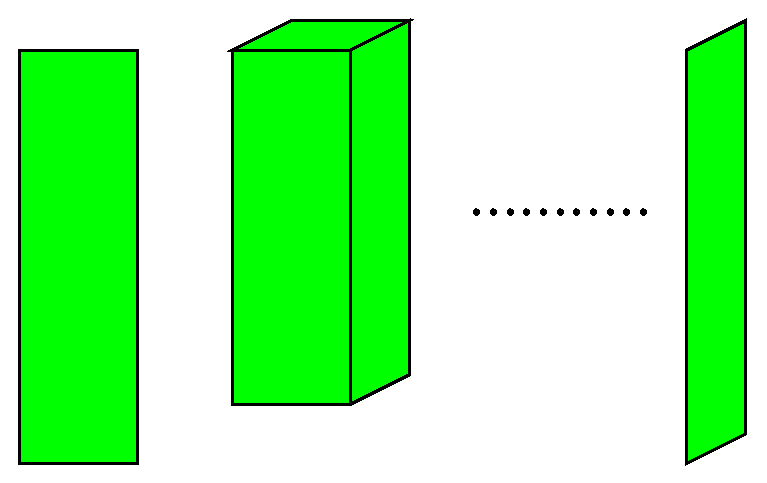
\includegraphics[scale=0.275]{./ttentry-simple.eps}
			\end{center}
			\end{block}
	\end{column}\hfill
	\begin{column}{0.325\linewidth}
	\begin{block}{\scriptsize Sequential algorithm}
		\begin{center}
			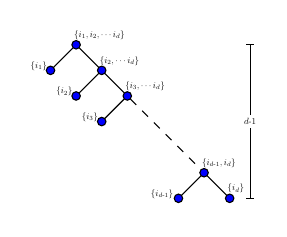
\begin{tikzpicture}[scale=0.325, every node/.style={transform shape}]
			%%\draw[fill=cyan] (0,0) circle (0.8cm);
			%%		\node [draw,circle]{r};
			%%		\tikzstyle{task}=[circle, draw, minimum size=10mm]
			%%		\node (d) at (0,0)[task, fill=babyblueeyes] {$D$};
			%%		\node (e) at (2.5,0)[task, fill=pastelviolet] {$E$};
			%%		\draw[thick, ->] (d.east) -- (e);
			%%		
			%%		\node (a) at (0,2)[task, fill=pastelyellow] {$A$};
			%%		\node (b) at (2.5,2.75)[task, fill=pastelgreen] {$B$};
			%%		\node (c) at (2.5,1.25)[task, fill=pastelred] {$C$};
			%%		
			%%		\draw[thick, ->] (a.east) -- (b);
			%%		\draw[thick, ->] (a.east) -- (c);
			\tikzstyle{taskc}=[circle, draw=black, minimum size=2mm, fill=blue]
			\tikzstyle{taskr}=[draw=none, minimum height=2mm, minimum width=5mm, anchor=south west, fill=none, text=black]
			%%
			\node (t01) at (0,0) [taskc]{};
			\node (t11) at (-1,-1) [taskc] {};
			\node (t12) at (1, -1) [taskc] {};
			\node (t21) at (0, -2) [taskc] {};
			\node (t22) at (2, -2) [taskc] {};
			\node (t31) at (1,-3) [taskc] {};
			\node (t52) at (5, -5) [taskc] {};
			\node (t61) at (4, -6) [taskc] {};
			\node (t62) at (6, -6) [taskc] {};
			
			\draw (t01) -- (t11);
			\draw (t01) -- (t12);
			\draw (t12) -- (t21);
			\draw (t12) -- (t22);
			\draw (t22) -- (t31);
			\draw [dashed] (t22) -- (t52);
			\draw (t52) -- (t61);
			\draw (t52) -- (t62);
			
			\draw (6.8, -6) -- (6.8, -3.25);
			\draw (6.8, -2.75) -- (6.8, 0);
			
			\draw (6.65, -6) -- (6.95, -6);
			\draw (6.65, -0) -- (6.95, 0);
			\node at (6.8, -3) {$d\text{-}1$};
			
			\node [above left=0mm and 2mm of t01.mid, taskr](l01) {$\{i_1,i_2,\cdots i_d\}$};
			\node [below left=2mm and 9mm of t11.mid, taskr](l11) {$\{i_1\}$};
			\node [above left=0mm and 2mm of t12.mid, taskr](l12) {$\{i_2,\cdots i_d\}$};
			\node [below left=2mm and 9mm of t21.mid, taskr](l21) {$\{i_2\}$};
			\node [above left=0mm and 2mm of t22.mid, taskr](l22) {$\{i_3,\cdots i_d\}$};
			\node [below left=2mm and 9mm of t31.mid, taskr](l31) {$\{i_3\}$};
			
			\node [above left=0mm and 2mm of t52.mid, taskr](l52) {$\{i_{d\text{-}1}, i_d\}$};
			\node [below left=2mm and 12mm of t61.mid, taskr](l61) {$\{i_{d\text{-}1}\}$};
			\node [above left=0mm and 2mm of t62.mid, taskr](l62) {$\{i_d\}$};
			
			\path (-0.1, -6.4) -- (2.5, -6.4); 
			\end{tikzpicture}
		\end{center}
	\end{block}
\end{column}\hfill
\begin{column}{0.325\linewidth}
	\begin{block}{\scriptsize For better parallelization}
		\begin{center}
			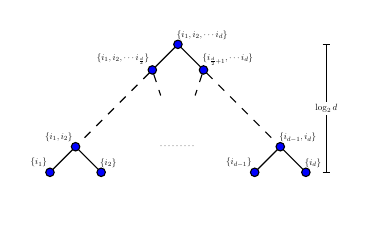
\begin{tikzpicture}[scale=0.325, every node/.style={transform shape}]
			
			\tikzstyle{taskc}=[circle, draw=black, minimum size=2mm, fill=blue]
			%%	\tikzstyle{taskr}=[draw=none, minimum height=2mm, minimum width=5mm, anchor=south west, fill=none, text=black]
			
			
			\node (t01) at (0,0) [taskc]{};
			\node (t11) at (-1,-1) [taskc] {};
			\node (t12) at (1, -1) [taskc] {};
			
			\node (tinter1) at (-0.5,-2) [taskc, draw=none, fill=none] {};
			\node (tinter2) at (0.5,-2) [taskc, draw=none, fill=none] {};
			
			\node (t41) at (-4,-4) [taskc] {};
			\node (t42) at (4,-4) [taskc] {};
			\node (t51) at (-5,-5) [taskc] {};
			\node (t52) at (-3,-5) [taskc] {};
			\node (t53) at (3,-5) [taskc] {};
			\node (t54) at (5,-5) [taskc] {};
			
			
			\draw (t01) -- (t11);
			\draw (t01) -- (t12);
			
			\draw [dashed] (t11) -- (tinter1.west);
			\draw [dashed] (t12) -- (tinter2.east);
			
			\draw [dashed] (t11) -- (t41);
			\draw [dashed] (t12) -- (t42);
			
			\path (t41) -- (t42) node [midway] {$\cdots\cdots\cdots$};
			
			\draw (t41) -- (t51);
			\draw (t41) -- (t52);
			
			\draw (t42) -- (t53);
			\draw (t42) -- (t54);
			
			
			\draw (5.8, -5) -- (5.8, -2.75);
			\draw (5.8, -2.25) -- (5.8, 0);
			
			\draw (5.65, -5) -- (5.95, -5);
			\draw (5.65, 0) -- (5.95, 0);
			\node at (5.8, -2.5) {$\log_2 d$};
			
			\node [above right] at (t01.160) {$\{i_1,i_2,\cdots i_d\}$};	
			
			\node [above left] at (t11.mid) {$\{i_1,i_2,\cdots i_\frac{d}{2}\}$};	
			\node [above right] at (t12.160) {$\{i_{\frac{d}{2}+1},\cdots i_d\}$};
			
			\node [above left] at (t41.mid) {$\{i_1,i_2\}$};
			\node [above right] at (t42.160) {$\{i_{d-1}, i_d\}$};
			
			\node [above left] at (t51.mid) {$\{i_1\}$};
			\node [above right] at (t52.160) {$\{i_2\}$};
			
			\node [above left] at (t53.mid) {$\{i_{d-1}\}$};
			\node [above right] at (t54.160) {$\{i_d\}$};
			
			
			\path (-0.1, -6.4) -- (2.5, -6.4); 
			%%		\path (-6.5, 0) -- (0,0);
			\end{tikzpicture}
		\end{center}
	\end{block}
\end{column}
\end{columns}
\end{block}
\vfill
\begin{block}{\footnotesize Communication Optimal Parallel Algorithms for Tensor Computations {\tiny (Inria, current)}}
	\begin{columns}
		\begin{column}{0.4\linewidth}
			\begin{itemize}
				\item Obtain $\Y$ from $\X, A, B, C$ 
				\item Obtain $\X$ from $\Y, A, B, C$ 
			\end{itemize}
		\end{column}
		\begin{column}{0.56\linewidth}\vspace*{-0.35cm}
			\begin{center}
				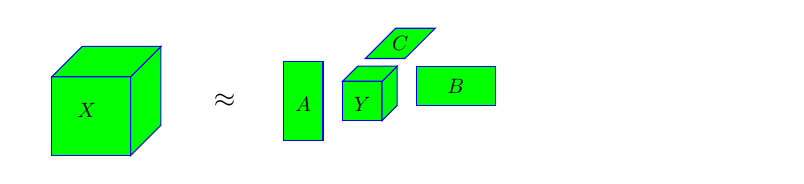
\begin{tikzpicture}[scale=0.25, every node/.style={transform shape}]
				\pgfmathsetmacro{\cubex}{4}
				\pgfmathsetmacro{\cubey}{4}
				\pgfmathsetmacro{\cubez}{4}
				\draw[blue,fill=pastelgreen] (-12,1,\cubez-2) -- ++(-\cubex,0,0) -- ++(0,-\cubey,0) -- ++(\cubex,0,0) -- cycle;
				\node [scale=3] at (-15,-1.5, 0) {$\X$};
				\draw[blue,fill=pastelgreen] (-12,1,\cubez-2) -- ++(0,0,-\cubez) -- ++(0,-\cubey,0) -- ++(0,0,\cubez) -- cycle;
				\draw[blue,fill=pastelgreen] (-12,1,\cubez-2) -- ++(-\cubex,0,0) -- ++(0,0,-\cubez) -- ++(\cubex,0,0) -- cycle;
				\node[draw=none, text=black, scale=4] at (-8,-1,0) {$\approx$};
				
				\pgfmathsetmacro{\cubex}{2}
				\pgfmathsetmacro{\cubey}{2}
				\pgfmathsetmacro{\cubez}{2}
				\draw[blue,fill=pastelgreen] (0,0,0) -- ++(-\cubex,0,0) -- ++(0,-\cubey,0) -- ++(\cubex,0,0) -- cycle;
				\draw[blue,fill=pastelgreen] (0,0,0) -- ++(0,0,-\cubez) -- ++(0,-\cubey,0) -- ++(0,0,\cubez) -- cycle;
				\draw[blue,fill=pastelgreen] (0,0,0) -- ++(-\cubex,0,0) -- ++(0,0,-\cubez) -- ++(\cubex,0,0) -- cycle;
				
				\node [scale=3] at (-1, -1.2, 0) {$\Y$};
				\draw[blue,fill=pastelgreen] (-\cubex-1,1,0) -- ++(-\cubex,0,0) -- ++(0,-\cubey-2,0) -- ++(\cubex,0,0) -- cycle;
				
				\node [scale=3] at (-4, -1.2, 0) {$A$};
				
				\draw[blue,fill=pastelgreen] (\cubex+2+1,0,-\cubey) -- ++(-\cubex-2,0,0) -- ++(0,-\cubey,0) -- ++(\cubex+2,0,0) -- cycle;
				\node [scale=3] at (3.75, -0.25, 0) {$B$};
				
				\draw[blue,fill=pastelgreen] (0,0,-\cubez-1) -- ++(-\cubex,0,0) -- ++(0,0,-\cubez-2) -- ++(\cubex,0,0) -- cycle;
				\node [scale=3] at (-1, 0, -5) {$C$};
				
				\path (-18,0) -- (20,0);
				\end{tikzpicture}
			\end{center}
		\end{column}
	\end{columns}
\end{block}
}

%%\begin{itemize}
%%	\item One item for tensor train
%%	\item Give a table for communication/computation time on supercomputers
%%	\item Tucker tensor decomposition
%%\end{itemize}
\end{frame}

%%\begin{frame}{Present Collaborations}
%%\begin{itemize}
%%	\item Parallel algorithms for high dimensional tensors -- with Laura Grigori (Inria Paris) and Olivier Beaumont (Inria Bordeaux)
%%	\vfill
%%	\item Communication optimal algorithms for Tensor computations -- with Laura Grigori, Grey Ballard (Wake Forest University, USA), Kathryn Rouse (Inmar Intelligence, USA) and Hussam Al Daas (STFC Rutherford Appleton Laboratory, UK)
%%	\vfill
%%	\item Theoretical models to perform molecular dynamics simulations with a few number of parameters -- with Laura Grigori, Yvon Maday (Sorbonne
%%	University), Eric Cances (Ecole des Ponts ParisTech) and Jean-Philip Piquemal (Sorbonne University)
%%	\vfill 
%%	\item Efficient implementation of density matrix renormalization group (DMRG) algorithm -- with Laura Grigori and Julien Toulouse (Sorbonne University)
%%\end{itemize}
%%\end{frame}


\part[Past/Ongoing Work]{Past/Ongoing Work}
%%\section{Introduction}
%%\begin{frame}{Outline}
%%\tableofcontents[currentsection]
%%\end{frame}



%%\begin{frame}{Tensors are used in Several Domains}
%%\begin{minipage}{0.575\linewidth}
%%	\begin{itemize}
%%		\item \textbf{Neuroscience}: Neuron $\times$ Time $\times$ Trial
%%		\item \textbf{Transportation}: Pickup $\times$ Dropoff $\times$ Time
%%		\item \textbf{Media}: User x Movie x Time 
%%		\item \textbf{Ecommerce}: User x Product x Time
%%	\end{itemize}
%%\end{minipage}
%%\begin{minipage}{0.4\linewidth}
%%	\begin{center}
%%		\begin{tikzpicture}[scale=0.125, every node/.style={transform shape}]
%%		\pgfmathsetmacro{\rectx}{4}
%%		\pgfmathsetmacro{\recty}{0.5}
%%		\draw[blue,fill=pastelgreen] (0,0) -- node [below, scale=6, black] {Vector}++(-\rectx,0) -- ++(0,\recty) -- ++(\rectx, 0) -- cycle;
%%		\end{tikzpicture}$\quad$
%%		\begin{tikzpicture}[scale=0.125, every node/.style={transform shape}]
%%		\pgfmathsetmacro{\rectx}{4}
%%		\pgfmathsetmacro{\recty}{4}
%%		\draw[blue,fill=pastelgreen] (0,0) -- node [below, scale=6, black] {Matrix}++(-\rectx,0) -- ++(0,\recty) -- ++(\rectx, 0) -- cycle;
%%		%%\addvmargin{4};
%%		\end{tikzpicture}$\ $
%%		\begin{tikzpicture}[scale=0.125, every node/.style={transform shape}]
%%		\pgfmathsetmacro{\cubex}{4}
%%		\pgfmathsetmacro{\cubey}{4}
%%		\pgfmathsetmacro{\cubez}{4}
%%		\draw[blue,fill=pastelgreen] (0,0,0) -- ++(-\cubex,0,0) -- ++(0,-\cubey,0) --node [below, scale=6, black] {3-dimensional tensor} ++(\cubex,0,0) -- cycle;
%%		\draw[blue,fill=pastelgreen] (0,0,0) -- ++(0,0,-\cubez) -- ++(0,-\cubey,0) -- ++(0,0,\cubez) -- cycle;
%%		\draw[blue,fill=pastelgreen] (0,0,0) -- ++(-\cubex,0,0) -- ++(0,0,-\cubez) -- ++(\cubex,0,0) -- cycle;
%%		\end{tikzpicture}
%%	\end{center}
%%	\begin{center}	
%%		\begin{tikzpicture}[scale=0.125, every node/.style={transform shape}]
%%		\pgfmathsetmacro{\cubex}{4}
%%		\pgfmathsetmacro{\cubey}{4}
%%		\pgfmathsetmacro{\cubez}{4}
%%		\draw[blue,fill=pastelgreen] (0,0,0) -- ++(-\cubex,0,0) -- ++(0,-\cubey,0) -- ++(\cubex,0,0) -- cycle;
%%		\draw[blue,fill=pastelgreen] (0,0,0) -- ++(0,0,-\cubez) -- ++(0,-\cubey,0) -- ++(0,0,\cubez) -- cycle;
%%		\draw[blue,fill=pastelgreen] (0,0,0) -- ++(-\cubex,0,0) -- ++(0,0,-\cubez) -- ++(\cubex,0,0) -- cycle;
%%		
%%		\draw[blue,fill=pastelgreen] (\cubex +2,0,0) -- ++(-\cubex,0,0) -- ++(0,-\cubey,0) -- ++(\cubex,0,0) -- cycle;
%%		\draw[blue,fill=pastelgreen] (\cubex +2,0,0) -- ++(0,0,-\cubez) -- ++(0,-\cubey,0) -- ++(0,0,\cubez) -- cycle;
%%		\draw[blue,fill=pastelgreen] (\cubex +2,0,0) -- ++(-\cubex,0,0) -- ++(0,0,-\cubez) -- ++(\cubex,0,0) -- cycle;
%%		
%%		\draw[blue,fill=pastelgreen] (\cubex +2 + \cubex +2,0,0) -- ++(-\cubex,0,0) -- ++(0,-\cubey,0) -- ++(\cubex,0,0) -- cycle;
%%		\draw[blue,fill=pastelgreen] (\cubex +2 + \cubex +2,0,0) -- ++(0,0,-\cubez) -- ++(0,-\cubey,0) -- ++(0,0,\cubez) -- cycle;
%%		\draw[blue,fill=pastelgreen] (\cubex +2 + \cubex +2,0,0) -- ++(-\cubex,0,0) -- ++(0,0,-\cubez) -- ++(\cubex,0,0) -- cycle;
%%		
%%		\draw[blue, fill=none] (-\cubex -1, 2.5, 0) -- ++(0, -\cubey -3.5, 0) --node [below, scale=6, black] {4-dimensional tensor} ++(\cubex +2 + \cubex +2 + \cubex + \cubex,0,0) -- ++(0, \cubey +3.5, 0) -- cycle; 
%%		
%%		%%\node [scale=2] at (0, -8) {$hello$};
%%		\end{tikzpicture}
%%	\end{center}
%%\end{minipage}
%%\vspace*{-0.2cm}
%%\begin{itemize}
%%	\item \textbf{Cyber-Traffic}: IP x IP x Port x Time
%%	\item \textbf{Social-Network}: Person x Person x Time x Interaction-Type
%%\end{itemize}
%%\begin{block}{High Dimensional Tensors}
%%	\begin{itemize}
%%		\item \textbf{Neural Network}: \begin{center}\vspace*{-0.35cm}
%%			\begin{tikzpicture}[scale=0.45, every node/.style={transform shape}]
%%			\tikzstyle{taskc}=[circle, draw=black, minimum size=2mm, fill=none]
%%			
%%			\node (t00) at (0,1) [taskc] {};
%%			\node (t01) at (0,0) [taskc] {};
%%			\node (t02) at (0,-1) [taskc] {};
%%			
%%			\draw (-0.5,1) -- (t00);
%%			\draw (-0.5,0) -- (t01);
%%			\draw (-0.5,-1) -- (t02);
%%			
%%			\node (t10) at (2,1.5) [taskc] {};
%%			\node (t11) at (2,0.5) [taskc] {};
%%			\node (t12) at (2,-0.5) [taskc] {};
%%			\node (t13) at (2,-1.5) [taskc] {};
%%			
%%			\draw (t00) -- (t10);
%%			\draw (t00) -- (t11);
%%			\draw (t00) -- (t12);
%%			\draw (t00) -- (t13);
%%			
%%			\draw (t01) -- (t10);
%%			\draw (t01) -- (t11);
%%			\draw (t01) -- (t12);
%%			\draw (t01) -- (t13);
%%			
%%			\draw (t02) -- (t10);
%%			\draw (t02) -- (t11);
%%			\draw (t02) -- (t12);
%%			\draw (t02) -- (t13);
%%			
%%			\node (t20) at (4,0.5) [taskc] {};
%%			\node (t21) at (4,-0.5) [taskc] {};
%%			
%%			\draw (t10) -- (t20);
%%			\draw (t10) -- (t21);
%%			
%%			\draw (t11) -- (t20);
%%			\draw (t11) -- (t21);
%%			
%%			\draw (t12) -- (t20);
%%			\draw (t12) -- (t21);
%%			
%%			\draw (t13) -- (t20);
%%			\draw (t13) -- (t21);
%%			
%%			\draw (t20) -- (4.5, 0.5);
%%			\draw (t21) -- (4.5, -0.5);
%%			%%	\node (t01) at (0,0) [taskc]{};
%%			%%	\draw (t01) -- (1,0);
%%			%%	\draw (t01) -- (-1,0);
%%			\path (6.8, 0) -- (9.0,0);
%%			\end{tikzpicture} 	
%%		\end{center}
%%		%%	\includegraphics[scale=0.02]{./tmp/neuralNetwork.jpg}
%%		\item \textbf{Molecular Simulation}: To represent wave functions
%%		\item \textbf{Quantum Computing}: Tensor network based models for computations
%%	\end{itemize}
%%\end{block}
%%\end{frame}


\begin{frame}{Tensors and Importance of Communication}
\vspace*{-0.1025cm}
\begin{minipage}{0.575\linewidth}
	\begin{itemize}
		\item[$\textcolor{blue}{\bullet}$] \textbf{Neuroscience}: Neuron $\times$ Time $\times$ Trial
%%		\item \textbf{Transportation}: Pickup $\times$ Dropoff $\times$ Time
		\item[$\textcolor{blue}{\bullet}$] \textbf{Media}: User x Movie x Time 
		\item[$\textcolor{blue}{\bullet}$] \textbf{Ecommerce}: User x Product x Time
		\item[$\textcolor{blue}{\bullet}$] \textbf{Social-Network}: Person x Person x Time x Type
	\end{itemize}
\end{minipage}
\begin{minipage}{0.4\linewidth}
	\begin{center}
		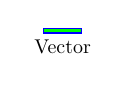
\begin{tikzpicture}[scale=0.12, every node/.style={transform shape}]
		\pgfmathsetmacro{\rectx}{4}
		\pgfmathsetmacro{\recty}{0.5}
		\draw[blue,fill=pastelgreen] (0,0) -- node [below, scale=6, black] {Vector}++(-\rectx,0) -- ++(0,\recty) -- ++(\rectx, 0) -- cycle;
		\end{tikzpicture}$\quad$
		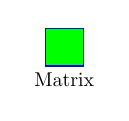
\begin{tikzpicture}[scale=0.12, every node/.style={transform shape}]
		\pgfmathsetmacro{\rectx}{4}
		\pgfmathsetmacro{\recty}{4}
		\draw[blue,fill=pastelgreen] (0,0) -- node [below, scale=6, black] {Matrix}++(-\rectx,0) -- ++(0,\recty) -- ++(\rectx, 0) -- cycle;
		%%\addvmargin{4};
		\end{tikzpicture}$\ $
		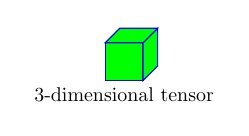
\begin{tikzpicture}[scale=0.12, every node/.style={transform shape}]
		\pgfmathsetmacro{\cubex}{4}
		\pgfmathsetmacro{\cubey}{4}
		\pgfmathsetmacro{\cubez}{4}
		\draw[blue,fill=pastelgreen] (0,0,0) -- ++(-\cubex,0,0) -- ++(0,-\cubey,0) --node [below, scale=6, black] {3-dimensional tensor} ++(\cubex,0,0) -- cycle;
		\draw[blue,fill=pastelgreen] (0,0,0) -- ++(0,0,-\cubez) -- ++(0,-\cubey,0) -- ++(0,0,\cubez) -- cycle;
		\draw[blue,fill=pastelgreen] (0,0,0) -- ++(-\cubex,0,0) -- ++(0,0,-\cubez) -- ++(\cubex,0,0) -- cycle;
		\end{tikzpicture}
	\end{center}
	\begin{center}	
		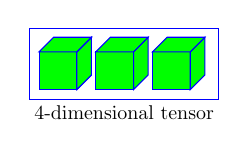
\begin{tikzpicture}[scale=0.12, every node/.style={transform shape}]
		\pgfmathsetmacro{\cubex}{4}
		\pgfmathsetmacro{\cubey}{4}
		\pgfmathsetmacro{\cubez}{4}
		\draw[blue,fill=pastelgreen] (0,0,0) -- ++(-\cubex,0,0) -- ++(0,-\cubey,0) -- ++(\cubex,0,0) -- cycle;
		\draw[blue,fill=pastelgreen] (0,0,0) -- ++(0,0,-\cubez) -- ++(0,-\cubey,0) -- ++(0,0,\cubez) -- cycle;
		\draw[blue,fill=pastelgreen] (0,0,0) -- ++(-\cubex,0,0) -- ++(0,0,-\cubez) -- ++(\cubex,0,0) -- cycle;
		
		\draw[blue,fill=pastelgreen] (\cubex +2,0,0) -- ++(-\cubex,0,0) -- ++(0,-\cubey,0) -- ++(\cubex,0,0) -- cycle;
		\draw[blue,fill=pastelgreen] (\cubex +2,0,0) -- ++(0,0,-\cubez) -- ++(0,-\cubey,0) -- ++(0,0,\cubez) -- cycle;
		\draw[blue,fill=pastelgreen] (\cubex +2,0,0) -- ++(-\cubex,0,0) -- ++(0,0,-\cubez) -- ++(\cubex,0,0) -- cycle;
		
		\draw[blue,fill=pastelgreen] (\cubex +2 + \cubex +2,0,0) -- ++(-\cubex,0,0) -- ++(0,-\cubey,0) -- ++(\cubex,0,0) -- cycle;
		\draw[blue,fill=pastelgreen] (\cubex +2 + \cubex +2,0,0) -- ++(0,0,-\cubez) -- ++(0,-\cubey,0) -- ++(0,0,\cubez) -- cycle;
		\draw[blue,fill=pastelgreen] (\cubex +2 + \cubex +2,0,0) -- ++(-\cubex,0,0) -- ++(0,0,-\cubez) -- ++(\cubex,0,0) -- cycle;
		
		\draw[blue, fill=none] (-\cubex -1, 2.5, 0) -- ++(0, -\cubey -3.5, 0) --node [below, scale=6, black] {4-dimensional tensor} ++(\cubex +2 + \cubex +2 + \cubex + \cubex,0,0) -- ++(0, \cubey +3.5, 0) -- cycle; 
		
		%%\node [scale=2] at (0, -8) {$hello$};
		\end{tikzpicture}
	\end{center}
\end{minipage}
%%\vspace*{-0.2cm}
%%\begin{itemize}
%%%%	\item \textbf{Cyber-Traffic}: IP x IP x Port x Time
%%	\item[$\textcolor{blue}{\bullet}$] \textbf{Social-Network}: Person x Person x Time x Interaction-Type
%%\end{itemize}
\begin{itemize}
	\item High dimensional tensors: Neural network, Molecular simulation, Quantum computing
	\item People work with low dimensional structure (decomposition) of the tensors
	\vspace*{-0.25cm}\begin{center}
\begin{columns}
	\hfill\begin{column}{0.285\linewidth}
		\begin{block}{\footnotesize Canonical decomposition}
				\begin{center}
				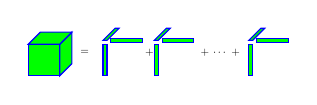
\begin{tikzpicture}[scale=0.1, every node/.style={transform shape}]
				\pgfmathsetmacro{\cubex}{4}
				\pgfmathsetmacro{\cubey}{4}
				\pgfmathsetmacro{\cubez}{4}
				\draw[blue,fill=pastelgreen] (0,0,0) -- ++(-\cubex,0,0) -- ++(0,-\cubey,0) -- ++(\cubex,0,0) -- cycle;
				\draw[blue,fill=pastelgreen] (0,0,0) -- ++(0,0,-\cubez) -- ++(0,-\cubey,0) -- ++(0,0,\cubez) -- cycle;
				\draw[blue,fill=pastelgreen] (0,0,0) -- ++(-\cubex,0,0) -- ++(0,0,-\cubez) -- ++(\cubex,0,0) -- cycle;
				
				\node[draw=none, text=black, scale=4] at (2,-2.25,-3) {$=$};
				\pgfmathsetmacro{\smallwidth}{0.5}
				\draw[blue,fill=pastelgreen] (\cubex+2,0,0) -- ++(-\smallwidth,0,0) -- ++(0,-\cubey,0) -- ++(\smallwidth,0,0) -- cycle;
				\draw[blue,fill=pastelgreen] (\cubex+2 +\cubex + 0.5,0.75,0) -- ++(-\cubex,0,0) -- ++(0,-\smallwidth,0) -- ++(\cubex,0,0) -- cycle;
				\draw[blue,fill=pastelgreen] (\cubex+2,0.5,0) -- ++(-\smallwidth,0,0) -- ++(0,0,-\cubez) -- ++(\smallwidth,0,0) -- cycle;
				
				\node[draw=none, text=black, scale=4] at (2+\cubex+4.25,-2.25,-3) {$+$};
				
				\draw[blue,fill=pastelgreen] (\cubex+2.5 + \cubex+2,0,0) -- ++(-\smallwidth,0,0) -- ++(0,-\cubey,0) -- ++(\smallwidth,0,0) -- cycle;
				\draw[blue,fill=pastelgreen] (\cubex+2.5+\cubex+2 +\cubex + 0.5,0.75,0) -- ++(-\cubex,0,0) -- ++(0,-\smallwidth,0) -- ++(\cubex,0,0) -- cycle;
				\draw[blue,fill=pastelgreen] (\cubex+2.5+\cubex+2,0.5,0) -- ++(-\smallwidth,0,0) -- ++(0,0,-\cubez) -- ++(\smallwidth,0,0) -- cycle;
				
				\node[draw=none, text=black, scale=4] at (2+\cubex+5 + \cubex+ 4.25, -2.25,-3) {$+$ $\cdots$ $+$};
				
				\draw[blue,fill=pastelgreen] (12 + \cubex+2.5 + \cubex+2,0,0) -- ++(-\smallwidth,0,0) -- ++(0,-\cubey,0) -- ++(\smallwidth,0,0) -- cycle;
				\draw[blue,fill=pastelgreen] (12+\cubex+2.5+\cubex+2 +\cubex + 0.5,0.75,0) -- ++(-\cubex,0,0) -- ++(0,-\smallwidth,0) -- ++(\cubex,0,0) -- cycle;
				\draw[blue,fill=pastelgreen] (12 + \cubex+2.5+\cubex+2,0.5,0) -- ++(-\smallwidth,0,0) -- ++(0,0,-\cubez) -- ++(\smallwidth,0,0) -- cycle;
				\end{tikzpicture}
			\end{center}
		\end{block}
	\end{column}
	\begin{column}{0.285\linewidth}
		\begin{block}{\footnotesize Tucker decomposition}
			\begin{center}
				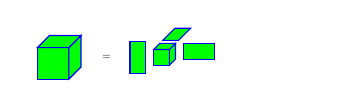
\begin{tikzpicture}[scale=0.1, every node/.style={transform shape}]
				\pgfmathsetmacro{\cubex}{4}
				\pgfmathsetmacro{\cubey}{4}
				\pgfmathsetmacro{\cubez}{4}
				\draw[blue,fill=pastelgreen] (-12,1,\cubez-2) -- ++(-\cubex,0,0) -- ++(0,-\cubey,0) -- ++(\cubex,0,0) -- cycle;
				\draw[blue,fill=pastelgreen] (-12,1,\cubez-2) -- ++(0,0,-\cubez) -- ++(0,-\cubey,0) -- ++(0,0,\cubez) -- cycle;
				\draw[blue,fill=pastelgreen] (-12,1,\cubez-2) -- ++(-\cubex,0,0) -- ++(0,0,-\cubez) -- ++(\cubex,0,0) -- cycle;
				\node[draw=none, text=black, scale=4] at (-8,-1,0) {$=$};
				
				\pgfmathsetmacro{\cubex}{2}
				\pgfmathsetmacro{\cubey}{2}
				\pgfmathsetmacro{\cubez}{2}
				\draw[blue,fill=pastelgreen] (0,0,0) -- ++(-\cubex,0,0) -- ++(0,-\cubey,0) -- ++(\cubex,0,0) -- cycle;
				\draw[blue,fill=pastelgreen] (0,0,0) -- ++(0,0,-\cubez) -- ++(0,-\cubey,0) -- ++(0,0,\cubez) -- cycle;
				\draw[blue,fill=pastelgreen] (0,0,0) -- ++(-\cubex,0,0) -- ++(0,0,-\cubez) -- ++(\cubex,0,0) -- cycle;
				
				\draw[blue,fill=pastelgreen] (-\cubex-1,1,0) -- ++(-\cubex,0,0) -- ++(0,-\cubey-2,0) -- ++(\cubex,0,0) -- cycle;
				\draw[blue,fill=pastelgreen] (\cubex+2+1,0,-\cubey) -- ++(-\cubex-2,0,0) -- ++(0,-\cubey,0) -- ++(\cubex+2,0,0) -- cycle;
				
				\draw[blue,fill=pastelgreen] (0,0,-\cubez-1) -- ++(-\cubex,0,0) -- ++(0,0,-\cubez-2) -- ++(\cubex,0,0) -- cycle;
				
				\path (-18,0) -- (20,0);
				\end{tikzpicture}
			\end{center}
		\end{block}
	\end{column}
	\begin{column}{0.285\linewidth}
		\begin{block}{\footnotesize Tensor Train decomposition}
				\begin{center}
				\begin{tikzpicture}[scale=0.1, every node/.style={transform shape}]
				
				\node (t0) at (0,-2.75) [scale=6] {$\tensor{X}$};
				\node [scale=4]at (2.5, -2.75) {$=$};
				\path (5,-6) -- (0,0);
				\end{tikzpicture}\hspace*{-0.15cm}
				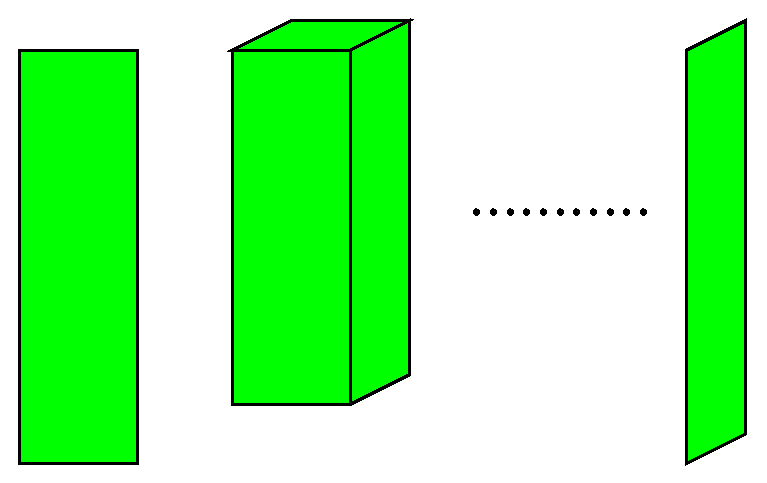
\includegraphics[scale=0.0825]{./ttentry-simple.eps}
			\end{center}
			
		\end{block}
	\end{column}
\end{columns}
	\end{center}
	\item Gaps between computation and communication growing exponentially on a parallel computer
{\footnotesize\begin{center}
	\begin{tabular}{|c|c|c|c|}
		\hline
		& time-per-operation & Network-bandwidth & Network-latency\\ \hline
		Annual improvements & 59 \% & 26 \% & 15 \%\\ \hline
		%%		\multicolumn{2}{|c|}{Annual improvements}\\ \hline
		%%		time-per-operation & 59\%\\ \hline
		%%		Network-bandwidth & 26\%\\ \hline
		%%		Network-latency & 15 \% \\ \hline
	\end{tabular}$\qquad\qquad\qquad$
\end{center}}
{$\ \;$\tiny Source: Getting up to speed: The future of supercomputing}
\end{itemize}
\end{frame}



%%\begin{frame}{Tensor Computations}
%%
%%{\small
%%	\begin{itemize}
%%		%%	\item Tensors are used in several domains
%%		%%	\begin{itemize}
%%		%%		\item Quantum molecular dynamics, signal processing, data mining, neurosciences, computer vision, psychometrics, chemometrics, ...
%%		%%	\end{itemize}
%%		%%	\vfill
%%		\item Memory and computation requirements are exponential in the number of dimensions
%%		\begin{itemize}
%%			\item A simulation involving just $100$ spatial orbitals manipulates a huge tensor with $4^{100}$ elements
%%			
%%		\end{itemize}
%%		\vfill
%%		\item People work with low dimensional structure (decomposition) of the tensors
%%		\begin{itemize}
%%			\item A tensor is represented with smaller objects
%%			%%		\item Useful to find patterns in massive data
%%			\item Improves memory and computation requirements
%%		\end{itemize}
%%		\vfill
%%		%%	\item Singular value decomposition (SVD) provides the most accurate low rank approximations for matrices
%%		%%	\vfill
%%		%%	\begin{itemize}
%%		%%		\item Most tensor decompositions are based on SVD of matricized tensors
%%		%%	\end{itemize} 
%%		%%	\vfill
%%		%%%%	\item Limited work on parallelization of tensor algorithms
%%		%%%%	
%%		%%%%	\vfill
%%		\item Most tensor decompositions rely on Singular Value Decomposition (SVD) of matrices
%%		%%	\item Singular Value Decomposition (SVD) provides the most accurate low rank approximations of matrices
%%		\begin{itemize}
%%			%%	\item It decomposes a matrix $A$ $\in$ $\mathbb{R}^{m \times n}$ to the form $U\Sigma V^T$
%%			%%	\begin{itemize}
%%			%%		\item $U$ is an $m\times m$ orthogonal matrix
%%			%%		\item $V$ is an $n\times n$ orthogonal matrix
%%			%%		\item $\Sigma$ is an $m\times n$ rectangular diagonal matrix
%%			%%	\end{itemize}
%%			\item SVD represents a matrix as the sum of rank one matrices, $A= U\Sigma V^T= \sum_i\Sigma(i;i)U_i V_i^T$
%%			%%%%	\begin{itemize}
%%			%%%%%%		\item $A= \sum_i \Sigma(i;i)U_i V_i^T$
%%			%%%%		\item Minimum number of rank one matrices required in the sum is called the rank of the matrix
%%			%%%%	\end{itemize}
%%			\begin{center}
%%				\begin{tikzpicture}[scale=0.2, every node/.style={transform shape}]
%%				\pgfmathsetmacro{\cubex}{4}
%%				\pgfmathsetmacro{\cubey}{4}
%%				\pgfmathsetmacro{\cubez}{4}
%%				\draw[blue,fill=pastelgreen] (0,0,0) -- ++(-\cubex,0,0) -- ++(0,-\cubey,0) -- ++(\cubex,0,0) -- cycle;
%%				%%\draw[blue,fill=pastelgreen] (0,0,0) -- ++(0,0,-\cubez) -- ++(0,-\cubey,0) -- ++(0,0,\cubez) -- cycle;
%%				%%\draw[blue,fill=pastelgreen] (0,0,0) -- ++(-\cubex,0,0) -- ++(0,0,-\cubez) -- ++(\cubex,0,0) -- cycle;
%%				
%%				\node[draw=none, text=black, scale=4] at (1.5,-3,-3) {$=$};
%%				
%%				\draw[blue,fill=pastelgreen] (6,0,0) -- ++(-\cubex+2.15,0,0) -- ++(0,-\cubey,0) -- ++(\cubex-2.15,0,0) -- cycle;
%%				
%%				\draw[blue,fill=pastelgreen] (10.25,0,0) -- ++(-\cubex,0,0) -- ++(0,-\cubey+2.15,0) -- ++(\cubex,0,0) -- cycle;
%%				
%%				\node[draw=none, text=black, scale=4] at (10.65,-3,-3) {$=$};
%%				
%%				\pgfmathsetmacro{\smallwidth}{0.5}
%%				\draw[blue,fill=pastelgreen] (9+\cubex+2,0,0) -- ++(-\smallwidth,0,0) -- ++(0,-\cubey,0) -- ++(\smallwidth,0,0) -- cycle;
%%				\draw[blue,fill=pastelgreen] (9+\cubex+2 +\cubex + 0.5,0.75,0) -- ++(-\cubex,0,0) -- ++(0,-\smallwidth,0) -- ++(\cubex,0,0) -- cycle;
%%				%%\draw[blue,fill=pastelgreen] (\cubex+2,0.5,0) -- ++(-\smallwidth,0,0) -- ++(0,0,-\cubez) -- ++(\smallwidth,0,0) -- cycle;
%%				
%%				\node[draw=none, text=black, scale=4] at (9+2+\cubex+4.25,-3,-3) {$+$};
%%				
%%				\draw[blue,fill=pastelgreen] (9+\cubex+2.5 + \cubex+2,0,0) -- ++(-\smallwidth,0,0) -- ++(0,-\cubey,0) -- ++(\smallwidth,0,0) -- cycle;
%%				\draw[blue,fill=pastelgreen] (9+\cubex+2.5+\cubex+2 +\cubex + 0.5,0.75,0) -- ++(-\cubex,0,0) -- ++(0,-\smallwidth,0) -- ++(\cubex,0,0) -- cycle;
%%				%%\draw[blue,fill=pastelgreen] (\cubex+2.5+\cubex+2,0.5,0) -- ++(-\smallwidth,0,0) -- ++(0,0,-\cubez) -- ++(\smallwidth,0,0) -- cycle;
%%				
%%				\node[draw=none, text=black, scale=4] at (9+2+\cubex+5 + \cubex+ 4.25, -3,-3) {$+$ $\cdots$ $+$};
%%				
%%				\draw[blue,fill=pastelgreen] (9+12 + \cubex+2.5 + \cubex+2,0,0) -- ++(-\smallwidth,0,0) -- ++(0,-\cubey,0) -- ++(\smallwidth,0,0) -- cycle;
%%				\draw[blue,fill=pastelgreen] (9+12+\cubex+2.5+\cubex+2 +\cubex + 0.5,0.75,0) -- ++(-\cubex,0,0) -- ++(0,-\smallwidth,0) -- ++(\cubex,0,0) -- cycle;
%%				%%\draw[blue,fill=pastelgreen] (12 + \cubex+2.5+\cubex+2,0.5,0) -- ++(-\smallwidth,0,0) -- ++(0,0,-\cubez) -- ++(\smallwidth,0,0) -- cycle;
%%				\end{tikzpicture}$\qquad\qquad\qquad\qquad$
%%			\end{center}
%%		\end{itemize}
%%		
%%		%%    \begin{itemize}
%%		%%    	\item Matricized Tensor Times Khatri Rao Product (MTTKRP), tensor contraction
%%		%%    \end{itemize}
%%	\end{itemize}
%%}
%%\end{frame}




%%\begin{frame}{Popular Tensor Decompositions (Higher Order Generalization of SVD)}
%%
%%{\small
%%%%\begin{block}{}
%%\vspace*{-0.25cm}
%%\begin{itemize}
%%	\item Canonical decomposition (Also known as Canonical Polyadic or CANDECOMP/PARAFAC)
%%	\begin{center}
%%		\begin{tikzpicture}[scale=0.2, every node/.style={transform shape}]
%%		\pgfmathsetmacro{\cubex}{4}
%%		\pgfmathsetmacro{\cubey}{4}
%%		\pgfmathsetmacro{\cubez}{4}
%%		\draw[blue,fill=pastelgreen] (0,0,0) -- ++(-\cubex,0,0) -- ++(0,-\cubey,0) -- ++(\cubex,0,0) -- cycle;
%%		\draw[blue,fill=pastelgreen] (0,0,0) -- ++(0,0,-\cubez) -- ++(0,-\cubey,0) -- ++(0,0,\cubez) -- cycle;
%%		\draw[blue,fill=pastelgreen] (0,0,0) -- ++(-\cubex,0,0) -- ++(0,0,-\cubez) -- ++(\cubex,0,0) -- cycle;
%%		
%%		\node[draw=none, text=black, scale=4] at (2,-2.25,-3) {$=$};
%%		\pgfmathsetmacro{\smallwidth}{0.5}
%%		\draw[blue,fill=pastelgreen] (\cubex+2,0,0) -- ++(-\smallwidth,0,0) -- ++(0,-\cubey,0) -- ++(\smallwidth,0,0) -- cycle;
%%		\draw[blue,fill=pastelgreen] (\cubex+2 +\cubex + 0.5,0.75,0) -- ++(-\cubex,0,0) -- ++(0,-\smallwidth,0) -- ++(\cubex,0,0) -- cycle;
%%		\draw[blue,fill=pastelgreen] (\cubex+2,0.5,0) -- ++(-\smallwidth,0,0) -- ++(0,0,-\cubez) -- ++(\smallwidth,0,0) -- cycle;
%%		
%%		\node[draw=none, text=black, scale=4] at (2+\cubex+4.25,-2.25,-3) {$+$};
%%		
%%		\draw[blue,fill=pastelgreen] (\cubex+2.5 + \cubex+2,0,0) -- ++(-\smallwidth,0,0) -- ++(0,-\cubey,0) -- ++(\smallwidth,0,0) -- cycle;
%%		\draw[blue,fill=pastelgreen] (\cubex+2.5+\cubex+2 +\cubex + 0.5,0.75,0) -- ++(-\cubex,0,0) -- ++(0,-\smallwidth,0) -- ++(\cubex,0,0) -- cycle;
%%		\draw[blue,fill=pastelgreen] (\cubex+2.5+\cubex+2,0.5,0) -- ++(-\smallwidth,0,0) -- ++(0,0,-\cubez) -- ++(\smallwidth,0,0) -- cycle;
%%		
%%		\node[draw=none, text=black, scale=4] at (2+\cubex+5 + \cubex+ 4.25, -2.25,-3) {$+$ $\cdots$ $+$};
%%		
%%		\draw[blue,fill=pastelgreen] (12 + \cubex+2.5 + \cubex+2,0,0) -- ++(-\smallwidth,0,0) -- ++(0,-\cubey,0) -- ++(\smallwidth,0,0) -- cycle;
%%		\draw[blue,fill=pastelgreen] (12+\cubex+2.5+\cubex+2 +\cubex + 0.5,0.75,0) -- ++(-\cubex,0,0) -- ++(0,-\smallwidth,0) -- ++(\cubex,0,0) -- cycle;
%%		\draw[blue,fill=pastelgreen] (12 + \cubex+2.5+\cubex+2,0.5,0) -- ++(-\smallwidth,0,0) -- ++(0,0,-\cubez) -- ++(\smallwidth,0,0) -- cycle;
%%		
%%		\end{tikzpicture}
%%	\end{center}
%%	%%\vfill
%%	\item Tucker decomposition
%%	\vspace*{-0.75cm}\begin{center}
%%		\begin{tikzpicture}[scale=0.2, every node/.style={transform shape}]
%%		\pgfmathsetmacro{\cubex}{4}
%%		\pgfmathsetmacro{\cubey}{4}
%%		\pgfmathsetmacro{\cubez}{4}
%%		\draw[blue,fill=pastelgreen] (-12,1,\cubez-2) -- ++(-\cubex,0,0) -- ++(0,-\cubey,0) -- ++(\cubex,0,0) -- cycle;
%%		\draw[blue,fill=pastelgreen] (-12,1,\cubez-2) -- ++(0,0,-\cubez) -- ++(0,-\cubey,0) -- ++(0,0,\cubez) -- cycle;
%%		\draw[blue,fill=pastelgreen] (-12,1,\cubez-2) -- ++(-\cubex,0,0) -- ++(0,0,-\cubez) -- ++(\cubex,0,0) -- cycle;
%%		\node[draw=none, text=black, scale=4] at (-8,-1,0) {$=$};
%%		
%%		\pgfmathsetmacro{\cubex}{2}
%%		\pgfmathsetmacro{\cubey}{2}
%%		\pgfmathsetmacro{\cubez}{2}
%%		\draw[blue,fill=pastelgreen] (0,0,0) -- ++(-\cubex,0,0) -- ++(0,-\cubey,0) -- ++(\cubex,0,0) -- cycle;
%%		\draw[blue,fill=pastelgreen] (0,0,0) -- ++(0,0,-\cubez) -- ++(0,-\cubey,0) -- ++(0,0,\cubez) -- cycle;
%%		\draw[blue,fill=pastelgreen] (0,0,0) -- ++(-\cubex,0,0) -- ++(0,0,-\cubez) -- ++(\cubex,0,0) -- cycle;
%%		
%%		\draw[blue,fill=pastelgreen] (-\cubex-1,1,0) -- ++(-\cubex,0,0) -- ++(0,-\cubey-2,0) -- ++(\cubex,0,0) -- cycle;
%%		\draw[blue,fill=pastelgreen] (\cubex+2+1,0,-\cubey) -- ++(-\cubex-2,0,0) -- ++(0,-\cubey,0) -- ++(\cubex+2,0,0) -- cycle;
%%		
%%		\draw[blue,fill=pastelgreen] (0,0,-\cubez-1) -- ++(-\cubex,0,0) -- ++(0,0,-\cubez-2) -- ++(\cubex,0,0) -- cycle;
%%		
%%		\path (-18,0) -- (20,0);
%%		\end{tikzpicture}
%%	\end{center}
%%	%%\vfill
%%	\item Tensor Train decomposition (equivalently known as Matrix Product States)
%%	
%%	\vspace*{-0.15cm}\begin{center}
%%		\begin{tikzpicture}[scale=0.2, every node/.style={transform shape}]
%%		
%%		\node (t0) at (0,-2.75) [scale=4] {$\tensor{A}$};
%%		\node [scale=4]at (2.5, -2.75) {$=$};
%%		\path (5,-6) -- (0,0);
%%		\end{tikzpicture}\hspace*{-0.15cm}
%%		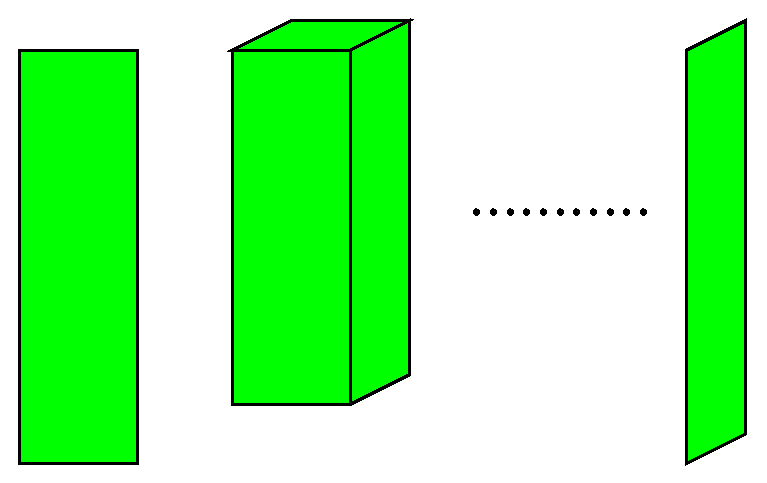
\includegraphics[scale=0.175]{./ttentry-simple.eps}$\qquad\qquad$
%%	\end{center}
%%\end{itemize}
%%}
%%\end{frame}
%%
%%
%%
%%\begin{frame}{Communication and its importance in HPC}
%%
%%\begin{minipage}{0.6\linewidth}
%%	\begin{itemize}
%%		\item Running time of an algorithm depends on 
%%		\begin{itemize}
%%			\item Computations
%%			\begin{itemize}
%%				\item Number of operations * time-per-operation
%%			\end{itemize}
%%			\item Data movement
%%			\begin{itemize}
%%				\item Volume of communication / Network-bandwidth
%%				\item Number of messages * Network-latency
%%			\end{itemize}
%%		\end{itemize}
%%	\end{itemize}
%%\end{minipage}
%%\begin{minipage}{0.35\linewidth}
%%	\begin{tikzpicture}[scale=0.625, every node/.style={transform shape}]
%%	%%\tikzstyle{taskmemory}=[draw=black, minimum height=18mm, minimum width=18mm, fill=blue!40, text=black]
%%	\tikzstyle{taskcompute}=[draw=black, minimum height=16mm, minimum width=16mm, fill=none, text=black, below]
%%	
%%	\node (t0) at (0,0) [taskcompute] {}; 
%%	\node (t1) at (4,0) [taskcompute] {};
%%	\node (t2) at (4,4) [taskcompute] {};
%%	\node (t3) at (0,4) [taskcompute] {};
%%	
%%	\draw [<->, line width=4, orange] (t0) -- (t1);
%%	\draw [<->, line width=4, orange] (t1) -- (t2);
%%	\draw [<->, line width=4, orange] (t2) -- (t3);
%%	\draw [<->, line width=4, orange] (t3) -- (t0);
%%	
%%	\node (td0)  at (t0.south) [above, scale=0.5] {$DRAM$};
%%	\node (td1) [above, scale=0.5] at (t1.south) {$DRAM$};
%%	\node (td2) [above, scale=0.5] at (t2.south) {$DRAM$};
%%	\node (td3) [above, scale=0.5] at (t3.south) {$DRAM$};
%%	
%%	\node [above] at (td0.north) {$CPU$};
%%	\node [above] at (td1.north) {$CPU$};
%%	\node [above] at (td2.north) {$CPU$};
%%	\node [above] at (td3.north) {$CPU$};
%%	
%%	%%\node [below] at (tm.south) {Memory Unit $M$};
%%	%%\node [above] at (tc.north) {Compute Unit $C$};
%%	%%
%%	%%\node [taskmemory, minimum height=6mm, minimum width=12mm, anchor=south] at (tc.south) {}; 
%%	\end{tikzpicture}
%%\end{minipage}
%%\begin{itemize}
%%	\item Gaps growing exponentially with time (Source: Getting up to speed: The future of supercomputing)
%%	\begin{center}
%%		\begin{tabular}{|c|c|c|c|}
%%			\hline
%%			& time-per-operation & Network-bandwidth & Network-latency\\ \hline
%%			Annual improvements & 59 \% & 26 \% & 15 \%\\ \hline
%%			%%		\multicolumn{2}{|c|}{Annual improvements}\\ \hline
%%			%%		time-per-operation & 59\%\\ \hline
%%			%%		Network-bandwidth & 26\%\\ \hline
%%			%%		Network-latency & 15 \% \\ \hline
%%		\end{tabular}
%%	\end{center}
%%	\vfill
%%	%%\credit{Getting up to speed: The future of supercomputing}
%%	\item Avoid communication to save time (and energy)
%%\end{itemize}
%%
%%
%%
%%%%\includegraphics[scale=0.02]{./tmp/networkTopology.jpg}
%%%%Source: GETTING UP TO SPEED THE FUTURE OF SUPERCOMPUTING
%%%%Figures fromGetting up to speed:  The future of supercomputing, 2005,National Academies Press (2004 figure based on data on the period 1988-2002)
%%\end{frame}


%%\begin{frame}
%%\frametitle{Previous Activities}
%%%%\tableofcontents[currentsection]
%%\tableofcontents
%%
%%
%%\begin{tikzpicture}[scale=0.625, every node/.style={transform shape}]
%%\tikzstyle{taskr}=[draw=black, rounded corners, minimum height=28mm, minimum width=86mm, fill=none, text=black]
%%
%%\path (0,0) --(1,0);
%%
%%
%%\node (otheractivities) at (4,0) [taskr, anchor=south] {};
%%
%%\node [below, align=left, text width=86mm]at (otheractivities.north) {
%%	\textbf{$\ $Other Significant Activities}:\medskip\\{\small
%%		\mybullet Performance optimizations on GPUs\\
%%		\mybullet Injecting static rules in dynamic schedulers\\
%%		\mybullet Large scale runtime systems\\
%%		\mybullet Communication lower bounds for computations}};
%%
%%\end{tikzpicture}
%%\end{frame}



\begin{frame}{Higher-order SVD (HOSVD) to compute Tucker decomposition}
\begin{center}
	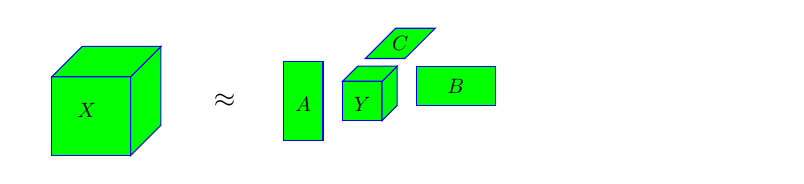
\begin{tikzpicture}[scale=0.25, every node/.style={transform shape}]
	\pgfmathsetmacro{\cubex}{4}
	\pgfmathsetmacro{\cubey}{4}
	\pgfmathsetmacro{\cubez}{4}
	\draw[blue,fill=pastelgreen] (-12,1,\cubez-2) -- ++(-\cubex,0,0) -- ++(0,-\cubey,0) -- ++(\cubex,0,0) -- cycle;
	\node [scale=3] at (-15,-1.5, 0) {$\X$};
	\draw[blue,fill=pastelgreen] (-12,1,\cubez-2) -- ++(0,0,-\cubez) -- ++(0,-\cubey,0) -- ++(0,0,\cubez) -- cycle;
	\draw[blue,fill=pastelgreen] (-12,1,\cubez-2) -- ++(-\cubex,0,0) -- ++(0,0,-\cubez) -- ++(\cubex,0,0) -- cycle;
	\node[draw=none, text=black, scale=4] at (-8,-1,0) {$\approx$};
	
	\pgfmathsetmacro{\cubex}{2}
	\pgfmathsetmacro{\cubey}{2}
	\pgfmathsetmacro{\cubez}{2}
	\draw[blue,fill=pastelgreen] (0,0,0) -- ++(-\cubex,0,0) -- ++(0,-\cubey,0) -- ++(\cubex,0,0) -- cycle;
	\draw[blue,fill=pastelgreen] (0,0,0) -- ++(0,0,-\cubez) -- ++(0,-\cubey,0) -- ++(0,0,\cubez) -- cycle;
	\draw[blue,fill=pastelgreen] (0,0,0) -- ++(-\cubex,0,0) -- ++(0,0,-\cubez) -- ++(\cubex,0,0) -- cycle;
	
	\node [scale=3] at (-1, -1.2, 0) {$\Y$};
	\draw[blue,fill=pastelgreen] (-\cubex-1,1,0) -- ++(-\cubex,0,0) -- ++(0,-\cubey-2,0) -- ++(\cubex,0,0) -- cycle;
	
	\node [scale=3] at (-4, -1.2, 0) {$A$};
	
	\draw[blue,fill=pastelgreen] (\cubex+2+1,0,-\cubey) -- ++(-\cubex-2,0,0) -- ++(0,-\cubey,0) -- ++(\cubex+2,0,0) -- cycle;
	\node [scale=3] at (3.75, -0.25, 0) {$B$};
	
	\draw[blue,fill=pastelgreen] (0,0,-\cubez-1) -- ++(-\cubex,0,0) -- ++(0,0,-\cubez-2) -- ++(\cubex,0,0) -- cycle;
	\node [scale=3] at (-1, 0, -5) {$C$};
	
	\path (-18,0) -- (20,0);
	\end{tikzpicture}
	
	{\footnotesize
		\begin{algorithm}[H]{\footnotesize
				\caption{HOSVD Algorithm($\X$, $R_1$, $R_2$, $R_3$)}
				\begin{algorithmic}[1]
					\STATE $A \leftarrow$ $R_1$ left singular vectors of $\X_{(1)}$
					\STATE $B \leftarrow$ $R_2$ left singular vectors of $\X_{(2)}$
					\STATE $C \leftarrow$ $R_3$ left singular vectors of $\X_{(3)}$
					\STATE $\Y = \X \times_1 A^\Tra \times_2 B^\Tra \times_3 C^\Tra$
					\STATE Return $\Y$, $A$, $B$, $C$
				\end{algorithmic}
		}\end{algorithm}
		
		\vspace*{-0.45cm}
		\begin{itemize}
			\item $\X$, $\Y$: 3-dimensional input and output tensors (or arrays) \& $A$, $B$, $C$: matrices
			\item $\X_{(i)}$: matricization of $\X$ ($i$th dimension represents rows and remaining dimensions represent columns)
			\item Multiple Tensor-Times-Matrix (Multi-TTM) computation: $\Y = \X \times_1 A^\Tra \times_2 B^\Tra \times_3 C^\Tra$
			\begin{itemize}
				\item To obtain full tensor, $\X = \Y \times_1 A \times_2 B \times_3 C$
			\end{itemize}
		\end{itemize}
	}
	%%	\begin{algorithm}[H]
	%%		\caption{\label{alg:3dmultittm}3-dimensional Parallel Atomic Multi-TTM}
	%%		\begin{algorithmic}[1]
	%%			\REQUIRE $\T{X}$, $\Mn{A}{1}$, $\Mn{A}{2}$, $\Mn{A}{3}$, $p_1 \times p_2 \times p_3 \times q_1 \times q_2 \times q_3$ logical processor grid
	%%			\ENSURE $\T{Y}$ such that $\Y = \X \times_1 {\Mn{A}{1}}^\Tra \times_2 {\Mn{A}{2}}^\Tra \times_3 {\Mn{A}{3}}^\Tra$
	%%			\STATE $(p_1^\prime, p_2^\prime, p_3^\prime, q_1^\prime, q_2^\prime, q_3^\prime)$ is my processor id
	%%			\STATE //All-gather input tensor $\T{X}$
	%%			\STATE $\T{X}_{p_1^\prime p_2^\prime p_3^\prime}$ = All-Gather($\T{X}$, $(p_1^\prime, p_2^\prime, p_3^\prime, *, *, *)$)\label{alg:3dmultittm:line:allGatherInputTensor}
	%%			\STATE //All-gather input matrices
	%%			\STATE $\Mn{A}{1}_{p_1^\prime q_1^\prime}$ = All-Gather($\Mn{A}{1}$, $(p_1^\prime, *, *, q_1^\prime, *, *)$)\label{alg:3dmultittm:line:allGatherMatrix1}
	%%			\STATE $\Mn{A}{2}_{p_2^\prime q_2^\prime}$ = All-Gather($\Mn{A}{2}$, $(*, p_2^\prime, *, *, q_2^\prime, *)$)\label{alg:3dmultittm:line:allGatherMatrix2}
	%%			\STATE $\Mn{A}{3}_{p_3^\prime q_3^\prime}$ = All-Gather($\Mn{A}{3}$, $(*, *, p_3^\prime, *, *, q_3^\prime)$)\label{alg:3dmultittm:line:allGatherMatrix3}
	%%			\STATE //Perform local Multi-TTM computation in a temporary tensor $\T{T}$
	%%			\STATE $\T{T}$ = Local-Multi-TTM($\T{X}_{p_1^\prime p_2^\prime p_3^\prime}$, $\Mn{A}{1}_{p_1^\prime q_1^\prime}$, $\Mn{A}{2}_{p_2^\prime q_2^\prime}$, $\Mn{A}{3}_{p_3^\prime q_3^\prime}$)\label{alg:3dmultittm:line:localcomputation}
	%%			\STATE //Reduce-scatter the output tensor in $\T{Y}_{q_1^\prime q_2^\prime q_3^\prime}$
	%%			\STATE Reduce-Scatter($\T{Y}_{q_1^\prime q_2^\prime q_3^\prime}$, $\T{T}$, $(*, *, *, q_1^\prime, q_2^\prime, q_3^\prime)$)\label{alg:3dmultittm:line:reduceScatterOutputTensor}
	%%		\end{algorithmic}
	%%	\end{algorithm}
\end{center}

%% $\X = \Y \times_1 {\Mn{A}{1}} \cdots \times_d {\Mn{A}{d}}$ to obtain the full tensor or as $\Y = \X \times_1 {\Mn{A}{1}}^\Tra \cdots \times_d {\Mn{A}{d}}^\Tra$
\end{frame}


\begin{frame}
\frametitle{Communication Lower Bounds and Communication Optimal Algorithms} % Table of contents slide, comment this block out to remove it
\tableofcontents % Throughout your presentation, if you choose to use \section{} and \subsection{} commands, these will automatically be printed on this slide as an overview of your presentation

\begin{block}{Assumptions}
	\begin{itemize}
		\item $P$ number of processors
		\item Each processor performs (asymptotically) equal amount of operations
		\item No redundant operations
		\item One copy of data is in the system
		\begin{itemize}
			\item $1/P$th amount of inputs (before the computation) and output (after the computation) on each processor  
		\end{itemize}
		\item Each processor has enough memory
	\end{itemize}
\end{block}
{\footnotesize This is joint work with Laura Grigori (Inria Paris, France), Grey Ballard (Wake Forest University, USA), Kathryn Rouse (Inmar Intelligence, USA), and Hussam Al Daas (Rutherford Appleton Laboratory, UK).}
\end{frame}

\section{For Matrix Matrix Multiplications}

%%\begin{frame}{Outline (Lower Bounds and Communication Optimal Algorithms)}
%%\tableofcontents[currentsection]
%%\end{frame}
\begin{frame}{Existing Lower Bounds for Matrix Matrix Multiplications}
\begin{itemize}
\item $C=AB$, where $A \in \mathbb{R}^{n_1\times n_2}, B \in \mathbb{R}^{n_2\times n_3}$, and $C \in \mathbb{R}^{n_1\times n_3}$
\item Let $d_1=\min(n_1,n_2,n_3) \le d_2=median(n_1,n_2,n_3) \le d_3 = \max(n_1,n_2,n_3)$
\end{itemize}

\begin{minipage}{0.7\linewidth}
\begin{block}{\small Existing Communication Lower Bounds (CARMA [IPDPS 2013])}
	\begin{center}
		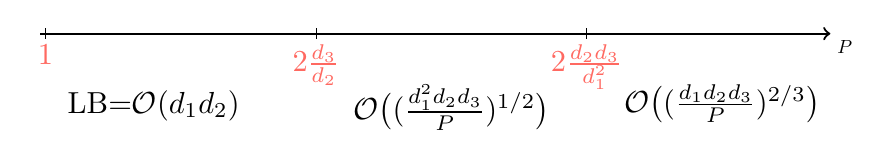
\begin{tikzpicture}[scale=0.6875, every node/.style={transform shape}]
		%%\draw (-2,0) -- node[below] {a} ++(2,0) -- node[above] {b} ++(2,0);
		%%\draw (-0.1,0) -- ++(5,0) -- ++(5,0);
		\draw [->, thick] (-0.1,0) -- (14.5,0) node [below right] {$P$};
		\draw (0, 0.1) -- node [below, pastelred, scale=1.6]{$1$}(0,-0.1);
		\draw (5, 0.1) -- node [below, pastelred, scale=1.6]{$2\frac{d_3}{d_2}$}(5,-0.1);
		\draw (10, 0.1) -- node [below, pastelred, scale=1.6] {$2\frac{d_2d_3}{d_1^2}$}(10,-0.1);
		
		\node[align=left,below,scale=1.6] at (2, -0.85) {LB=$\mathcal{O}(d_1d_2)$};
		\node[align=left,below,scale=1.6] at (7.5, -0.75) {$\mathcal{O}\big((\frac{d_1^2d_2d_3}{P})^{1/2}\big)$};
		\node[align=center,below,scale=1.6] at (12.5, -0.75) {$\mathcal{O}\big((\frac{d_1d_2d_3}{P})^{2/3}\big)$};	
		\end{tikzpicture}
	\end{center} 
\end{block}
{\begin{alertblock}{\small Our Communication Lower Bounds}
		\begin{center}
			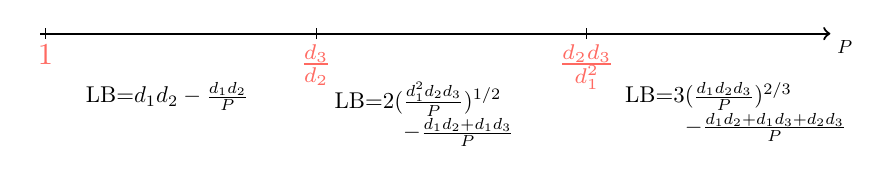
\begin{tikzpicture}[scale=0.6875, every node/.style={transform shape}]
			%%\draw (-2,0) -- node[below] {a} ++(2,0) -- node[above] {b} ++(2,0);
			%%\draw (-0.1,0) -- ++(5,0) -- ++(5,0);
			\draw [->, thick] (-0.1,0) -- (14.5,0) node [below right] {$P$};
			\draw (0, 0.1) -- node [below, pastelred, scale=1.6]{$1$}(0,-0.1);
			\draw (5, 0.1) -- node [below, pastelred, scale=1.6]{$\frac{d_3}{d_2}$}(5,-0.1);
			\draw (10, 0.1) -- node [below, pastelred, scale=1.6] {$\frac{d_2d_3}{d_1^2}$}(10,-0.1);
			
			\node[align=left,below,scale=1.2] at (2.25, -0.75) {LB=$d_1d_2 -\frac{d_1d_2}{P}$};
			\node[align=left,below,scale=1.2] at (7, -0.75) {LB=$2(\frac{d_1^2d_2d_3}{P})^{1/2}$\\
				$\qquad\quad-\frac{d_1d_2+d_1d_3}{P}$};
			\node[align=center,below,scale=1.2] at (12.25, -0.75) {LB=$3(\frac{d_1d_2d_3}{P})^{2/3}$\\ $\qquad\qquad\quad -\frac{d_1d_2+d_1d_3+d_2d_3}{P}$};	
			\end{tikzpicture}
		\end{center} 
\end{alertblock}}
\end{minipage}$\quad$
\begin{minipage}{0.25\linewidth}
\begin{exampleblock}{\small Arrangements of $8$ processors}
	\begin{center}
		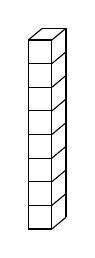
\begin{tikzpicture}[scale=0.3, every node/.style={transform shape}]	
		\foreach \x in {0, 1, 2, 3, 4, 5, 6, 7, 8}
		\draw (-1, \x) -- (0, \x);
		
		\foreach \x in {0, 1, 2, 3, 4, 5, 6, 7, 8}
		\draw (0, \x)--(0.6, 0.5+\x);
		
		\draw (0,0) -- (0,8);
		\draw(-1,0)--(-1,8);
		\draw (0.6,0.5) -- (0.6,8.5);
		\draw (-1,8) -- (-1+0.6,8.5);
		
		\draw (-1+0.6,8.5) -- (0.6,8.5);
		
		\end{tikzpicture}$\quad$
		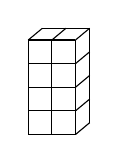
\begin{tikzpicture}[scale=0.3, every node/.style={transform shape}]
		
		\foreach \x in {0, 1, 2, 3, 4}
		\draw (-2, \x) -- (0, \x);
		
		\foreach \x in {0, 1, 2, 3, 4}
		\draw (0, \x)--(0.6, 0.5+\x);
		
		\draw (0,0) -- (0,4);
		\draw (-1,0) -- (-1,4);
		\draw(-2,0)--(-2,4);
		
		\draw (0.6,0.5) -- (0.6,4.5);
		
		\draw (-2,4) -- (-2+0.6, 4+0.5);
		\draw (-2+0.6, 4+0.5) -- (0.6, 4.5);
		
		\draw (-1,4) -- (-1+0.6, 4+0.5);
		
		%%\draw (-1,8) -- (0,8.5);
		%%\draw (0,8.5) -- (1,8.5);
		
		\end{tikzpicture}$\quad$
		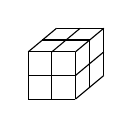
\begin{tikzpicture}[scale=0.3, every node/.style={transform shape}]
		
		\def\xref{0.6}
		\def\yref{0.5}
		
		\foreach \x in {0, 1, 2}
		\draw (-2, \x) -- (0, \x);
		
		\foreach \x in {0, 1, 2}
		\draw (0, \x)--(2*\xref, 2*\yref+\x);
		
		\draw (0,0) -- (0,2);
		\draw (-1,0) -- (-1,2);
		\draw (-2,0)--(-2,2);
		\draw (\xref,\yref) -- (\xref, 2+\yref);
		\draw (2*\xref,2*\yref) -- (2*\xref, 2+ 2*\yref);
		
		\draw (-2,2) -- (-2+2*\xref, 2+2*\yref);
		\draw (-1,2) -- (-1+2*\xref, 2+2*\yref);
		
		\draw (-2+2*\xref, 2+2*\yref) -- (2*\xref, 2+2*\yref);
		\draw (-2+\xref, 2+\yref) -- (\xref, 2+\yref);
		\end{tikzpicture}
	\end{center}
\end{exampleblock}
\end{minipage}
\end{frame}
\begin{frame}{Loomis-Whitney \&  H\"{o}lder-Brascamp-Lieb inequalities}
\vspace*{-0.25cm}\begin{block}{\small Size of $d-1$ dimensional projections (Loomis-Whitney inequalitiy)}
\begin{minipage}{0.375\linewidth}
\vspace*{-0.35cm}\begin{block}{}
	\begin{columns}
		\begin{column}{0.6\linewidth}
			\vspace*{-0.45cm}\begin{itemize}{\footnotesize
					\item $2$-dimensional object $A$ and its $1$-dimensional projections $\phi_x$, $\phi_y$
					\item $\phi_x \phi_y \ge Area(A)$
			}\end{itemize}		
		\end{column}
		\begin{column}{0.35\linewidth}
			\begin{center}
				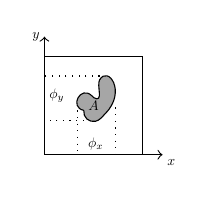
\begin{tikzpicture}[scale=0.25, every node/.style={transform shape}]
				\draw (0,0) -- ++(5,0) -- ++(0, 5) -- ++(-5,0) -- cycle;
				\draw [<->] (0,6) -- (0,0) -- (6,0);
				\node [below right, scale=2] at (6,0) {$x$};
				\node [left, scale=2] at (0,6) {$y$};
				
				\draw [fill=gray!70] (2,2.25) to [curve through={(2.4,3) .. (2.5,2.9) .. (2.8,3.8) .. (3.1,2.1) .. (2.6,1.7)}] (2,2.25);
				
				\node [scale=2] at (2.5,2.5) {$A$};
				\draw [dotted] (1.7,2.25) -- (1.7,0);
				\draw [dotted] (3.6,2.4) -- (3.6,0);
				
				\node[above, scale=2] at (2.6,0) {$\phi_x$};
				
				\draw [dotted] (2,1.75) -- (0,1.75);
				\draw [dotted] (2.8,4) -- (0,4);
				
				\node[right, scale=2] at (0,3) {$\phi_y$};
				\end{tikzpicture}
			\end{center}
		\end{column}
	\end{columns}
	
	%%		\vspace*{-0.75cm}
\end{block}
\end{minipage}$\quad$
\begin{minipage}{0.56\linewidth}
\vspace*{-0.35cm}\begin{block}{}
	\begin{columns}
		\begin{column}{0.6\linewidth}
			\vspace*{-0.4cm}\begin{itemize}{\footnotesize
					\item $3$-dimensional object $A$ and its $2$-dimensional projections: $\phi_{xy}$, $\phi_{yz}$, $\phi_{xz}$
					\item $(\phi_{xy}\phi_{yz}\phi_{xz})^\frac{1}{3-1} \ge Volume(A)$
			}\end{itemize}
		\end{column}
		\begin{column}{0.35\linewidth}
			\begin{center}
				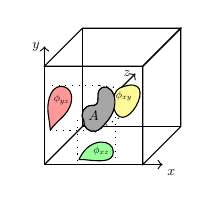
\begin{tikzpicture}[scale=0.25, every node/.style={transform shape}]
				\draw (0,0) -- ++(5,0) -- ++(0, 5) -- ++(-5,0) -- cycle;
				\draw (0,5,0) -- ++(0,0, -5) -- ++(5,0,0) -- ++(0,0,5) -- cycle;
				\draw (5,0,0) -- ++(0,0,-5) -- ++(0,5,0) -- ++(0,0,5) -- cycle;
				\draw (0,0,-5) -- ++(5,0,0) -- ++(0,5,0) -- ++(-5,0,0) -- cycle;
				\draw [<->] (0,6) -- (0,0) -- (6,0);
				\draw [->] (0,0,0) -- (0,0,-12);
				\node [left, scale=2, rotate=0] at (0,0,-12) {$z$};
				\node [below right, scale=2] at (6,0) {$x$};
				\node [left, scale=2] at (0,6) {$y$};
				
				\draw [fill=gray!70] (2,2.25) to [curve through={(2.4,3) .. (2.5,3) .. (2.8,3.8) .. (3.1,2.1) .. (2.6,1.7)}] (2,2.25);
				
				\node [scale=2] at (2.5,2.5) {$A$};
				\draw [dotted] (1.7,2.25) -- (1.7,0.2);
				\draw [dotted] (3.6,2.4) -- (3.6,0.3);
				
				\draw [fill=green!40] (1.75,0.25) to [curve through={(1.8, 0.35) .. (3.5, 0.65) .. (2,0.25)}] (1.75,0.25);
				\node[above, scale=1.5] at (2.6,0,-0.75) {$\phi_{xz}$};
				
				\draw [dotted] (2,1.75) -- (0.3,1.75);
				\draw [dotted] (2.8,4) -- (0.385,4);
				
				\draw [fill=red!40] (0.3, 1.75) to [curve through={(0.5,2) .. (1, 2.5) .. (1,3.95) .. (0.2, 2.5)}] (0.3,1.75);
				\node[right, scale=1.5] at (0,3, -0.75) {$\phi_{yz}$};
				
				\draw [fill=yellow!40] (3.85,3.9) to [curve through={(3.7,3.8) .. (3.5,3.4) .. (3.45,3.2)}] (3.85, 3.9);
				\node [scale=1.5] at (3.65,3.1,-1) {$\phi_{xy}$};
				\draw [dotted] (2.8,4) -- (3.8,3.9);
				\draw [dotted] (2.56,1.65) -- (4,2.5);
				
				\draw [fill=gray!70] (2,2.25) to [curve through={(2.4,3) .. (2.5,3) .. (2.8,3.8) .. (3.1,2.1) .. (2.6,1.7)}] (2,2.25);
				
				\node [scale=2] at (2.5,2.5) {$A$};
				\end{tikzpicture}
			\end{center}
		\end{column}
	\end{columns}
	%%		\vspace*{-0.85cm}
\end{block}
\end{minipage}\vspace*{-0.1cm}
\end{block}
\vspace*{-0.325cm}\begin{block}{\small H\"{o}lder-Brascamp-Lieb (HBL) inequality -- Generalization of Loomis-Whitney inequality}
\begin{columns}
\begin{column}{0.35\linewidth}{\small
		\vspace*{-0.5cm}\begin{center}
			$\M{\Delta} = \begin{blockarray}{cccc}
			& A & B & C  \\
			\begin{block}{c(ccc)}
			i & 1 & 0 & 1\\
			j & 0 & 1 & 1\\
			k & 1 & 1 & 0\\
			\end{block}
			\end{blockarray}$
		\end{center}
}\end{column}
\begin{column}{0.6\linewidth}
	\vspace*{-0.35cm}\begin{align*}
	&\text{for $i = 1{:}n_1$, for $k = 1{:}n_2$, for $j = 1{:}n_3$}\\
	&\quad \quad C[i][j] += A[i][k]*B[k][j]
	\end{align*}
\end{column}
\end{columns}
\vspace*{-0.6cm}\begin{itemize}{\small
	\item Find $\V{x}=\begin{bmatrix} x_1 & x_2 & x_3 \end{bmatrix}^\Tra$ such that $\M{\Delta}.\V{x} \ge \V{1}$, $\V{1}$ is vector of all ones
	\item $\phi_A, \phi_B, \phi_C$: projections of computations on arrays $A$, $B$, $C$
	\item HBL inequality:  $\phi_A^{x_1} \phi_B^{x_2} \phi_C^{x_3} \ge \text{Amount of computations}$
	\item To make inequality tight select $\V{x}$ such that $\V{1}^\Tra \V{x}$ is minimum $=>x_1=x_2=x_3 = \frac{1}{2}$ 
}\end{itemize}\vspace*{-0.25cm}	
\end{block}

%%\begin{tikzpicture}[scale=0.3, every node/.style={transform shape}]
%%%%\draw[help lines] (0,0) grid[step=0.25] (1,1);
%%%%\draw
%%%%(0,0) to [curve through={
%%%%	(0.15,0.35) .. 
%%%%	(0.5,0.5)   .. 
%%%%	(0.8,0.6) } ]  
%%%%(1,1);
%%
%%\draw [fill=gray!10] (0,0) to [curve through={(3.5,5) .. (4,5.2) .. (4.2,5.3) .. (5,5)}] (0,0);
%%
%%%%	\draw[blue,fill=pastelgreen] (\cubex+2+1,0,-\cubey) -- ++(-\cubex-2,0,0) -- ++(0,-\cubey,0) -- ++(\cubex+2,0,0) -- cycle;
%%\end{tikzpicture}

\end{frame}

\begin{frame}{Constraints for Matrix Multiplications}
\vspace*{-0.45cm}\begin{center}
\begin{align*}
&\text{for $i = 1{:}n_1$, for $k = 1{:}n_2$, for $j = 1{:}n_3$}\\
&\quad \quad C[i][j] += A[i][k]*B[k][j]
\end{align*}
\end{center}
\vspace{-0.25cm}\begin{itemize}
\item Total number of multiplications = $n_1n_2n_3$
\item Consider a processor which performs $\frac{n_1n_2n_3}{P}$ amount of multiplications
\item Optimization problem: \vspace*{-0.56cm}\begin{align*}
Minimize &\ \phi_A + \phi_B + \phi_C \  \text{ s.t.}\\
\phi_A^\frac{1}{2} \phi_B^\frac{1}{2}  \phi_C^\frac{1}{2} & \ge \frac{n_1n_2n_3}{P}
\end{align*}
\end{itemize}
\begin{block}{Extra constraints (our contributions)}
\begin{itemize}
\item Each element of $A$ (resp. $B$) is involved in $n_3$ (resp. $n_1$) multiplications
\begin{itemize}
\item To perform at least $\frac{n_1n_2n_3}{P}$ multiplications: $\phi_A \ge \frac{n_1n_2}{P}, \phi_B \ge \frac{n_2n_3}{P}$
\end{itemize}
\item Each element of $C$ is the sum of $n_2$ multiplications, therefore $\phi_C \ge \frac{n_1n_3}{P}$
\item Projections can be at max the size of the arrays: $\phi_A \le n_1n_2, \phi_B \le n_2n_3, \phi_C \le n_1n_3$ 
\end{itemize}
\end{block}
\end{frame}

\begin{frame}{Optimization Problem to Compute Communication Lower Bounds}

{\small$\bullet$ Projections ($\phi_A,  \phi_B, \phi_C$) indicate the amount of array access\\
$\bullet$ Communication lower bound = $\phi_A + \phi_B + \phi_C - \text{data owned by the processor}$
\begin{minipage}{0.45\linewidth}
\begin{center}
\begin{align*}
Minimize &\ \phi_A + \phi_B + \phi_C \  \text{ s.t.}\\
\phi_A^\frac{1}{2} \phi_B^\frac{1}{2}  \phi_C^\frac{1}{2} & \ge \frac{n_1n_2n_3}{P}\\
\frac{n_1n_2}{P} \le &\phi_A \le n_1n_2\\
\frac{n_2n_3}{P} \le &\phi_B \le n_2n_3\\
\frac{n_1n_3}{P} \le &\phi_C \le n_1n_3
\end{align*}
\end{center}
\end{minipage}
\begin{minipage}{0.5\linewidth}
\vspace*{-0.15cm}\begin{block}{Generalized version (in terms of $d_1$, $d_2$, $d_3$)}
\vspace*{-0.35cm}\begin{align*}
Minimize &\ \phi_1 + \phi_2 + \phi_3 \  \text{ s.t.}\\
\phi_1^\frac{1}{2} \phi_2^\frac{1}{2}  \phi_3^\frac{1}{2} & \ge \frac{d_1d_2d_3}{P}\\
\frac{d_1d_2}{P} \le &\phi_1 \le d_1d_2\\
\frac{d_1d_3}{P} \le &\phi_2 \le d_1d_3\\
\frac{d_2d_3}{P} \le &\phi_3 \le d_2d_3\\
d_1 \le & d_2 \le d_3
\end{align*}
\end{block}
\end{minipage}


}\end{frame}
\begin{frame}{Amount of Accesses and Communication Lower bounds}
$\bullet$ Estimate the solution based on Lagrange multipliers\\
$\bullet$ Prove optimality using all Karush–Kuhn–Tucker (KKT) conditions are satisfied
\begin{block}{\small Amount of accesses =$\phi_1 + \phi_2 + \phi_3$}
\begin{center}
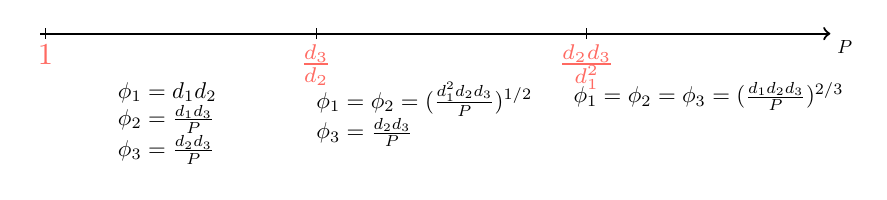
\begin{tikzpicture}[scale=0.6875, every node/.style={transform shape}]
%%\draw (-2,0) -- node[below] {a} ++(2,0) -- node[above] {b} ++(2,0);
%%\draw (-0.1,0) -- ++(5,0) -- ++(5,0);
\draw [->, thick] (-0.1,0) -- (14.5,0) node [below right] {$P$};
\draw (0, 0.1) -- node [below, pastelred, scale=1.6]{$1$}(0,-0.1);
\draw (5, 0.1) -- node [below, pastelred, scale=1.6]{$\frac{d_3}{d_2}$}(5,-0.1);
\draw (10, 0.1) -- node [below, pastelred, scale=1.6] {$\frac{d_2d_3}{d_1^2}$}(10,-0.1);

\node[align=left,below,scale=1.2] at (2.25, -0.75) {$\phi_1 = d_1d_2$\\ $\phi_2=\frac{d_1d_3}{P}$\\ $\phi_3 = \frac{d_2d_3}{P}$};
\node[align=left,below,scale=1.2] at (7, -0.75) {$\phi_1 =\phi_2= (\frac{d_1^2d_2d_3}{P})^{1/2}$\\ $\phi_3 = \frac{d_2d_3}{P}$};
\node[align=center,below,scale=1.2] at (12.25, -0.75) {$\phi_1 = \phi_2 = \phi_3 = (\frac{d_1d_2d_3}{P})^{2/3}$};	
\end{tikzpicture}
\end{center} 
\end{block}
\begin{block}{\small Communication Lower Bounds (Amount of Data Transfers)}
\begin{center}
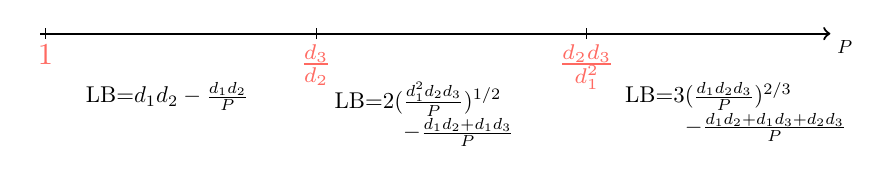
\begin{tikzpicture}[scale=0.6875, every node/.style={transform shape}]
%%\draw (-2,0) -- node[below] {a} ++(2,0) -- node[above] {b} ++(2,0);
%%\draw (-0.1,0) -- ++(5,0) -- ++(5,0);
\draw [->, thick] (-0.1,0) -- (14.5,0) node [below right] {$P$};
\draw (0, 0.1) -- node [below, pastelred, scale=1.6]{$1$}(0,-0.1);
\draw (5, 0.1) -- node [below, pastelred, scale=1.6]{$\frac{d_3}{d_2}$}(5,-0.1);
\draw (10, 0.1) -- node [below, pastelred, scale=1.6] {$\frac{d_2d_3}{d_1^2}$}(10,-0.1);

\node[align=left,below,scale=1.2] at (2.25, -0.75) {LB=$d_1d_2 -\frac{d_1d_2}{P}$};
\node[align=left,below,scale=1.2] at (7, -0.75) {LB=$2(\frac{d_1^2d_2d_3}{P})^{1/2}$\\
$\qquad\quad-\frac{d_1d_2+d_1d_3}{P}$};
\node[align=center,below,scale=1.2] at (12.25, -0.75) {LB=$3(\frac{d_1d_2d_3}{P})^{2/3}$\\ $\qquad\qquad\quad -\frac{d_1d_2+d_1d_3+d_2d_3}{P}$};	
\end{tikzpicture}
\end{center}
\end{block}
\end{frame}


\begin{frame}{Design of Communication Optimal Algorithms}
\vspace*{-0.25cm}\begin{block}{\small Data Distribution ($P$ is organized into a $p_1 \times p_2 \times p_3$ grid)}
\begin{minipage}{0.585\linewidth}{\small	
\begin{itemize}
\item Select $p_1,p_2$, and $p_3$ based on the lower bounds
\item Each processor has $\frac{1}{P}$th amount of $A$, $B$ and $C$
\item $A_{11} = A(1:\frac{n_1}{p_1}, 1:\frac{n_2}{p_2})$ is evenly distributed among $(1,1, *)$ processors
\item Similar data distributions for $B$ and $C$
\end{itemize}
}\end{minipage}
\begin{minipage}{0.4\linewidth}
	\begin{center}
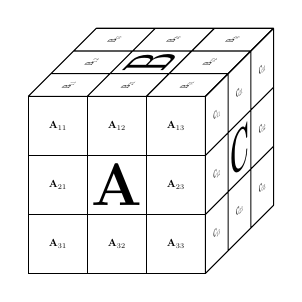
\begin{tikzpicture}[every node/.append style={transform shape},scale=0.75]
% draw lines signifying collectives
%%\draw[line width=3,stealth-stealth,red!75] (.1,2,0) -- (.1,2,-2.25);
%%\draw[line width=3,stealth-stealth,red!75] (0,2,0) -- (-2.25,2,0);
%%\draw[line width=3,stealth-stealth,red!75] (0,2,0) -- (0,-.25,0);
% right face of comp cube
\begin{scope}[canvas is yz plane at x=.5,rotate=-90,yscale=-1,shift={(-.5,-3+.5)}]
%%\draw[fill=red!25] (0,0) rectangle (1,1);
%%\draw[fill=red!75] (2/3,0) rectangle (1,1);
\draw[black] (0,0) grid (3,3);
%%\draw[black,xscale=1/3,dotted] (0,0) grid (3,1);
\node[yscale=-1,scale=2] at (3/2,3/2) {\Large $\CC$};
\node[yscale=-1,scale=.5] at (1/2,1/2) {$\CC_{11}$};
\node[yscale=-1,scale=.5] at (1/2,3/2) {$\CC_{12}$};
\node[yscale=-1,scale=.5] at (1/2,5/2) {$\CC_{13}$};
\node[yscale=-1,scale=.5] at (3/2,1/2) {$\CC_{21}$};
\node[yscale=-1,scale=.5] at (3/2,5/2) {$\CC_{23}$};
\node[yscale=-1,scale=.5] at (5/2,1/2) {$\CC_{31}$};
\node[yscale=-1,scale=.5] at (5/2,3/2) {$\CC_{32}$};
\node[yscale=-1,scale=.5] at (5/2,5/2) {$\CC_{33}$};
\end{scope}
% front face of comp cube
\begin{scope}[canvas is yx plane at z=.5,yscale=-1,rotate=180,shift={(-3+.5,-3+.5)}]
%%\draw[fill=red!25] (0,2) rectangle (1,3);
%%\draw[fill=red!75] (0,2) rectangle (1,7/3);
\draw[black] (0,0) grid (3,3);
%%\draw[black,shift={(0,2)},yscale=1/3,dotted] (0,0) grid (1,3);
\node[rotate=90,scale=2] at (3/2,3/2) {\Large $\A$};
\node[rotate=90,scale=.5] at (1/2,1/2) {$\A_{11}$};
\node[rotate=90,scale=.5] at (1/2,3/2) {$\A_{12}$};
\node[rotate=90,scale=.5] at (1/2,5/2) {$\A_{13}$};
\node[rotate=90,scale=.5] at (3/2,1/2) {$\A_{21}$};
\node[rotate=90,scale=.5] at (3/2,5/2) {$\A_{23}$};
\node[rotate=90,scale=.5] at (5/2,1/2) {$\A_{31}$};
\node[rotate=90,scale=.5] at (5/2,3/2) {$\A_{32}$};
\node[rotate=90,scale=.5] at (5/2,5/2) {$\A_{33}$};
\end{scope}
% top face of comp cube
\begin{scope}[canvas is zx plane at y=(3-.5),rotate=90,shift={(-3+.5,-.5)}]
%%\draw[fill=red!25] (2,0) rectangle (3,1);
%%\draw[fill=red!75] (2,0) rectangle (3,1/3);
\draw[black] (0,0) grid (3,3);
%%\draw[black,shift={(2,0)},yscale=1/3,dotted] (0,0) grid (1,3);
\node[rotate=90,scale=2] at (3/2,3/2) {\Large $\B$};
\node[rotate=90,scale=.5] at (1/2,1/2) {$\B_{11}$};
\node[rotate=90,scale=.5] at (1/2,3/2) {$\B_{12}$};
\node[rotate=90,scale=.5] at (1/2,5/2) {$\B_{13}$};
\node[rotate=90,scale=.5] at (3/2,1/2) {$\B_{21}$};
\node[rotate=90,scale=.5] at (3/2,5/2) {$\B_{23}$};
\node[rotate=90,scale=.5] at (5/2,1/2) {$\B_{31}$};
\node[rotate=90,scale=.5] at (5/2,3/2) {$\B_{32}$};
\node[rotate=90,scale=.5] at (5/2,5/2) {$\B_{33}$};
\end{scope}
\end{tikzpicture}
	\end{center}
\end{minipage}
\end{block}

\vspace*{-0.3cm}\begin{algorithm}[H]{\footnotesize
\caption{$C=AB$ Matrix Multiplication Algorithm}
\begin{algorithmic}[1]
\STATE $(p_1^\prime, p_2^\prime, p_3^\prime)$ is my processor id
\STATE //All-gather input matrices $A$ and $B$
\STATE $A_{p_1^\prime p_2^\prime}$ = All-Gather($A$, $(p_1^\prime, p_2^\prime, *)$)
\STATE $B_{p_2^\prime p_3^\prime}$ = All-Gather($B$, $(*, p_2^\prime, p_3^\prime)$)
%%			\STATE //Perform local Matrix Multiplication in a temporary variable $T$
\STATE $T$ = Local-Matrix-Multiplication($A_{p_1^\prime p_2^\prime}, B_{p_2^\prime p_3^\prime} $) // Local matrix multiplication in a temporary
%%			\STATE //Reduce-scatter the output matrix in $C_{p_1^\prime p_3^\prime}$
\STATE Reduce-Scatter($C_{p_1^\prime p_3^\prime}$, T,  $(p_1^\prime,*,p_3^\prime)$) // Reduce-scatter the output
\end{algorithmic}
}\end{algorithm}
\end{frame}
%%\begin{frame}{Cost Analysis and Open Questions}
%%\begin{block}{Cost Analysis}
%%\begin{itemize}
%%\item Total amount of multiplications per processor = $\frac{n_1n_2n_3}{p_1p_2p_3} = \frac{n_1n_2n_3}{P}$
%%%%		\item Amount of data transfers to perform All-Gather/Reduce-Scatter operation on $Q$ processors = $(1-\frac{1}{Q})w$, $w$ is amount of total data after All-Gather or before Reduce-Scatter operation
%%\item Total data transfers = $\frac{n_1n_2}{p_1p_2} + \frac{n_2n_3}{p_2p_3} + \frac{n_1n_3}{p_1p_3} - \frac{n_1n_2+n_2n_3+n_1n_3}{P}$   
%%\end{itemize}
%%\end{block}
%%\vfill
%%\begin{block}{Open Questions}
%%\begin{itemize}
%%\item How to select $p_1, p_2, p_3$?
%%\item Are communication lower bounds are achievable for all matrix dimensions?
%%\end{itemize}
%%\end{block}
%%
%%\end{frame}
%%
\section{For Multi-TTM Computation}
%%
%%\begin{frame}{Outline}
%%\tableofcontents
%%\end{frame}
%%\setcounter{algorithm}{0}
%%\begin{frame}{$3$-dimensional Multi-TTM Computation ($\Y = \X \times_1 {\Mn{A}{1}}^\Tra \times_2 {\Mn{A}{2}}^\Tra \times_3 {\Mn{A}{3}}^\Tra$)}
%%\begin{itemize}
%%%%\item $\T{X} \in \mathbb{R}^{n_1\times \cdots \times n_d}$: input tensor, $\T{Y}\in \mathbb{R}^{r_1\times\cdots \times r_d}$: output tensor
%%%%\item $\Mn{A}{k}\in \mathbb{R}^{n_k\times r_k}$: factor matrix of the $k$th mode
%%\item TTM-in-Sequence approach (used in Tucker-MPI)
%%\begin{itemize}
%%	\item For 2-dimensional computation, $\M{Y} = \MnTra{A}{1}{}\M{X}\Mn{A}{2}$
%%\end{itemize}  
%%\end{itemize}
%%\begin{block}{\small 2-dimensional Multi-TTM ($\Y = \X \times_1 {\Mn{A}{1}}^\Tra \times_2 {\Mn{A}{2}}^\Tra$)}
%%TTM-in-Sequence approach (used in Tucker-MPI): $\M{Y} = \MnTra{A}{1}{}\M{X}\Mn{A}{2}$\\
%%All-at-Once approach (our contribution):	
%%\vspace*{-0.25cm}\begin{align*}
%%&\text{for $n_1^\prime = 1{:}n_1$, for $n_2^\prime = 1{:}n_2$}\\
%%&\quad \text{for $r_1^\prime = 1{:}r_1$, for $r_2^\prime = 1{:}r_2$}\\
%%&\quad \quad \Y(r_1^\prime,r_2^\prime) = \Y(r_1^\prime,r_2^\prime) + \Big( \X(n_1^\prime,n_2^\prime) *  \Mn{A}{1}(n_{1}^\prime,r_1^\prime) * \Mn{A}{2}(n_2^\prime,r_2^\prime) \Big)
%%\end{align*}
%%\end{block}
%%
%%%%\begin{itemize}
%%%%	\item TTM-in-sequence
%%%%	\item All-at-once definition
%%%%\end{itemize}
%%\end{frame}

\begin{frame}{3-dimensional Multi-TTM ($\Y = \X \times_1 {\Mn{A}{1}}^\Tra \times_2 {\Mn{A}{2}}^\Tra \times_3 {\Mn{A}{3}}^\Tra$)}
\begin{itemize}
	\item TTM-in-Sequence approach (used in Tucker-MPI)
	\begin{itemize}
		\item For 2-dimensional computation, $\M{Y} = \MnTra{A}{1}{}\M{X}\Mn{A}{2}$
	\end{itemize}
	\item $\X: n_1\times n_2\times n_3$, $\Y:r_1 \times r_2 \times r_3$, $\Mn{A}{k}: n_k\times r_k$ 
\end{itemize}
\begin{block}{\small All-at-Once approach (our contribution)}
\begin{minipage}{0.7\linewidth}{\small
\vspace*{-0.25cm}\begin{align*}
&\text{for $n_1^\prime = 1{:}n_1$, for $n_2^\prime = 1{:}n_2$, for $n_3^\prime = 1{:}n_3$}\\
&\quad \text{for $r_1^\prime = 1{:}r_1$, for $r_2^\prime = 1{:}r_2$, for $r_3^\prime = 1{:}r_3$}\\
&\quad \quad \Y(r_1^\prime,r_2^\prime,r_3^\prime) = \Y(r_1^\prime,r_2^\prime,r_3^\prime)\\
&\qquad\qquad + \Big( \X(n_1^\prime,n_2^\prime,n_3^\prime) *  \Mn{A}{1}(n_{1}^\prime,r_1^\prime) * \Mn{A}{2}(n_2^\prime,r_2^\prime) * \Mn{A}{3}(n_3^\prime,r_3^\prime)\Big)
\end{align*}
}\end{minipage}
\begin{minipage}{0.25\linewidth}{\small
$\M{\Delta} = \begin{bmatrix}\M{I}_{3\times 3} & \V{1}_3 & \V{0}_3\\ \M{I}_{3\times 3} & \V{0}_3 & \V{1}_3 \end{bmatrix}$
}\end{minipage}
\end{block}
\begin{itemize}
\item Total number of inner ($4-array$) operations = $n_1r_1n_2r_2n_3r_3$
\item $\M{\Delta}$ is not full rank: allows us to get multiple constraints related to computations
\item Possible to solve matrix and tensor optimization problems separately
%%consider each $\V{x}$ such that $\M{\Delta}\cdot\V{x}=\V{1}$
%%\begin{itemize}
%%\item Consider each vector $\V{x}$ such that $\M{\Delta}\cdot\V{x}=\V{1}$, $\V{x}$ is of the form [$a$ $a$ $a$ $1$-$a$ $1$-$a$]$^\Tra$ and $0\le a\le 1$
%%\end{itemize}
%%\item $\phi_{\X}$, $\phi_{\Y}$: tensor projections \& $\phi_1, \phi_2, \phi_3$: matrix projections
%%\item From HBL, $\phi_{\X}^{1-a}\phi_{\Y}^{1-a} \phi_1^a \phi_2^a \phi_3^a \ge \text{Amount of computations}$, $0\le a\le 1$
\end{itemize}
\end{frame}

%%\begin{frame}{Solving Optimization Problem to Compute Lower Bounds}
%%\begin{itemize}
%%\item Select a processor which performs $\frac{n_1r_1n_2r_2n_3r_3}{P}$ amount of $4-array$ operations
%%\item After applying lower and upper bounds for each projection, we need to solve the following optimization problem
%%\end{itemize}
%%\vspace*{-0.35cm}\begin{align*}
%%Minimize \ \phi_{\X} + \phi_{\Y} +& \phi_1 + \phi_2 + \phi_3 \  \text{ s.t.}\\
%%\phi_{\X}^{1-a}\phi_{\Y}^{1-a} \phi_1^a \phi_2^a \phi_3^a & \ge \frac{n_1r_1n_2r_2n_3r_3}{P}\\
%%\frac{n_1n_2n_3}{P} \le & \phi_{\X} \le n_1n_2n_3\\
%%\frac{r_1r_2r_3}{P} \le & \phi_{\Y} \le r_1r_2r_3\\
%%\frac{n_1r_1}{P} \le &\phi_1 \le n_1r_1\\
%%\frac{n_2r_2}{P} \le &\phi_2 \le n_2r_2\\
%%\frac{n_3r_3}{P} \le &\phi_3 \le n_3r_3
%%\end{align*}
%%\end{frame}
%%\begin{frame}{Divide the problem into two parts}
%%\vspace*{-0.25cm}
%%\begin{minipage}{0.45\linewidth}
%%\begin{block}{Matrix part}{\small
%%\vspace*{-0.45cm}\begin{align*}
%%Minimize \ & \phi_1 + \phi_2 + \phi_3 \  \text{ s.t.}\\
%%\phi_1 \phi_2 \phi_3 & \ge \frac{n_1r_1n_2r_2n_3r_3}{P}\\
%%\frac{n_1r_1}{P} \le &\phi_1 \le n_1r_1\\
%%\frac{n_2r_2}{P} \le &\phi_2 \le n_2r_2\\
%%\frac{n_3r_3}{P} \le &\phi_3 \le n_3r_3
%%\end{align*}
%%}\end{block}
%%\end{minipage}$\quad$
%%\begin{minipage}{0.45\linewidth}
%%\begin{block}{Tensor part}{\small
%%\begin{align*}
%%Minimize \ & \phi_{\X} + \phi_{\Y}\  \text{ s.t.}\\
%%\phi_{\X}\phi_{\Y} & \ge \frac{n_1r_1n_2r_2n_3r_3}{P}\\
%%\frac{n_1n_2n_3}{P} \le & \phi_{\X} \le n_1n_2n_3\\
%%\frac{r_1r_2r_3}{P} \le & \phi_{\Y} \le r_1r_2r_3
%%\end{align*}
%%}\end{block}
%%\end{minipage}
%%
%%
%%\end{frame}
\begin{frame}{Amount of Accesses and Lower bounds}

\vspace*{-0.25cm}\begin{block}{Amount of accesses = $\phi_{\X} + \phi_{\Y} + \phi_1 + \phi_2 + \phi_3$}
\begin{center}
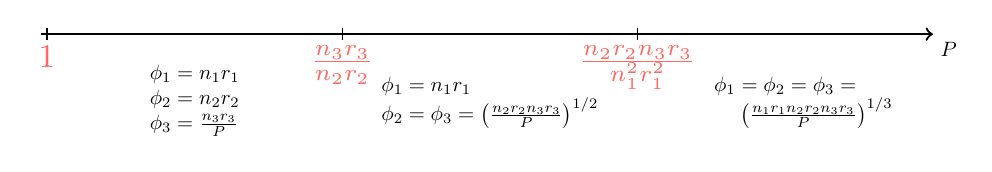
\begin{tikzpicture}[scale=0.75, every node/.style={transform shape}]
%%\draw (-2,0) -- node[below] {a} ++(2,0) -- node[above] {b} ++(2,0);
%%\draw (-0.1,0) -- ++(5,0) -- ++(5,0);
\draw [->, thick] (-0.1,0) -- (15,0) node [below right] {$P$};
\draw (0, 0.1) -- node [below, pastelred, scale=1.6]{$1$}(0,-0.1);
\draw (5, 0.1) -- node [below, pastelred, scale=1.6]{$\frac{n_3r_3}{n_2r_2}$}(5,-0.1);
\draw (10, 0.1) -- node [below, pastelred, scale=1.6] {$\frac{n_2r_2n_3r_3}{n_1^2r_1^2}$}(10,-0.1);

\node[align=left,below] at (2.5, -0.4) {$\phi_1=n_1r_1$\\ $\phi_2=n_2r_2$\\ $\phi_3=\frac{n_3r_3}{P}$};
\node[align=left,below] at (7.5, -0.6) {$\phi_1=n_1r_1$\\$\phi_2=\phi_3= \big(\frac{n_2r_2n_3r_3}{P}\big)^{1/2}$};
\node[align=center,below] at (12.5, -0.6) {$\phi_1=\phi_2=\phi_3=$\\ $\qquad\quad \big(\frac{n_1r_1n_2r_2n_3r_3}{P}\big)^{1/3}$};	
\end{tikzpicture}
\end{center}

\begin{center}
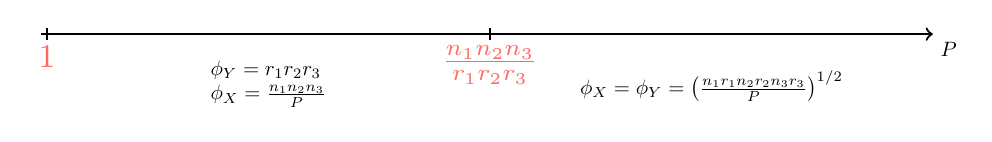
\begin{tikzpicture}[scale=0.75, every node/.style={transform shape}]
\draw [->, thick] (-0.1,0) -- (15,0) node [below right] {$P$};
\draw (0, 0.1) -- node [below, pastelred, scale=1.6]{$1$}(0,-0.1);
\draw (7.5, 0.1) -- node [below, pastelred, scale=1.6]{$\frac{n_1n_2n_3}{r_1r_2r_3}$}(7.5,-0.1);

\node[align=left,below] at (3.75, -0.325) {$\phi_{\Y}= r_1r_2r_3$\\ $\phi_{\X} = \frac{n_1n_2n_3}{P}$};
\node[align=left,below] at (11.25, -0.5) {$\phi_{\X}=\phi_{\Y}= \big(\frac{n_1r_1n_2r_2n_3r_3}{P}\big)^{1/2}$};
\end{tikzpicture}
\end{center}
\end{block}
\begin{itemize}{\small
		\item We assume $n_1r_1\le n_2r_2\le n_3r_3$ and $r_1r_2r_3\le n_1n_2n_3$
		%%\item Estimate solutions for both parts using Lagrange multipliers ( optimality can be proven using KKT conditions) 
		\item Communication lower bound = $\phi_{\X} + \phi_{\Y} + \phi_1 + \phi_2 + \phi_3 -\frac{n_1n_2n_3+r_1r_2r_3+n_1r_1+n_2r_2+n_3r_3}{P}$
		\item Can design similar communical optimal algorithm (though $6$-dimensional) for this
		\item Selection of optimal processor grid dimensions based on the lower bound requires some adaption
}\end{itemize}

\end{frame}
%%\begin{frame}{Design of Communication Optimal Algorithms}
%%\begin{block}{\small Data Distribution ($P$ is organized into a $p_1 \times p_2 \times p_3\times q_1 \times q_2 \times q_3$ grid)}{\small
%%%%		\begin{minipage}{0.75\linewidth}{\small	
%%\begin{itemize}
%%\item $p_1,p_2, p_3, q_1, q_2$, and $q_3$ evenly distribute $n_1, n_2, n_3, r_1, r_2$, and  $r_3$
%%\item Each processor has $\frac{1}{P}$th amount of input and output variables
%%\item Subtensor $\T{X}_{231} = \T{X}(\frac{n_1}{p_1}+1:2\frac{n_1}{p_1}, 2\frac{n_2}{p_2}+1:3\frac{n_2}{p_2}, 1:\frac{n_3}{p_3})$ is distributed evenly among processors $(2,3,1,*,*,*)$ 
%%\item Submatrix $\Mn{A}{2}_{31} = \Mn{A}{2}(2\frac{n_2}{p_2}+1:3\frac{n_2}{p_2}, 1:\frac{r_2}{q_2})$ is distributed evenly among processors $(*,3,*,*,1,*)$
%%\end{itemize}
%%%%		}\end{minipage}
%%\begin{center}
%%\vspace*{-0.25cm}\begin{tikzpicture}[scale=0.4, every node/.style={transform shape}]
%%\def\xref{0.6}
%%\def\yref{0.5}
%%
%%\foreach \y in {0, 1, 2, 3, 4}
%%\draw (-2, \y) -- (2, \y);
%%
%%\foreach \x in {-2, -1, 0, 1, 2}
%%\draw (\x, 0) -- (\x, 4);
%%
%%\foreach \y in {0, 1, 2, 3, 4}
%%\draw (2, \y)--(2+4*\xref, 4*\yref+\y);
%%
%%
%%\foreach \y in {0, 1, 2, 3, 4}
%%\draw (2+\y * \xref, \y * \yref) -- (2+\y * \xref, 4+\y * \yref);
%%
%%\foreach \x in {-2, -1, 0, 1, 2}
%%\draw (\x, 4) -- (\x + 4*\xref, 4+4*\yref);
%%
%%\foreach \y in {0, 1, 2, 3, 4}
%%\draw (-2+\y * \xref, 4+\y * \yref) -- (2+\y * \xref, 4+\y * \yref);
%%
%%\node [below, pastelgreen, scale=2.5] at (0,0) {$\T{X}$};
%%
%%\draw [dotted] (-1, 3) -- (-1+\xref,3+\yref);
%%\draw [dotted] (0, 3) -- (0+\xref,3+\yref);
%%\draw [dotted] (0, 2) -- (0+\xref,2+\yref);
%%\draw [dotted] (-1+\xref,3+\yref) -- (0+\xref,3+\yref);
%%\draw [dotted] (0+\xref,3+\yref) -- (0+\xref,2+\yref);
%%
%%\node [ pastelgreen, scale=1.2] at (-0.5,2.5) {$\T{X}_{231}$};
%%
%%\draw [->, red] (-1,-1.5) -- (1,-1.5) node [below right, scale=1.2] {$n_1$};
%%\draw [->, red] (-2.5,1) -- (-2.5,3) node [ above left, scale=1.2] {$n_2$};
%%\draw [->, red] (-2.5+\xref, 4+\yref) -- (-2.5 + 3*\xref, 4+3*\yref) node [above,rotate=45, scale=1.2] {$n_3$};
%%\end{tikzpicture}$\qquad$
%%\vspace*{-0.25cm}\begin{tikzpicture}[scale=0.4, every node/.style={transform shape}]
%%\def\xref{0.6}
%%\def\yref{0.5}
%%
%%\foreach \y in {0, 1, 2, 3, 4}
%%\draw (-2, \y) -- (2, \y);
%%
%%\foreach \x in {-2, -1, 0, 1, 2}
%%\draw (\x, 0) -- (\x, 4);
%%
%%\node [below, pastelgreen, scale=2.5] at (0,0) {$\Mn{A}{2}$};
%%
%%
%%\node [ pastelgreen, scale=1.2] at (-1.5,2.5) {$\Mn{A}{2}_{31}$};
%%
%%\draw [->, red] (-1,-1.5) -- (1,-1.5) node [below right, scale=1.2] {$r_2$};
%%\draw [->, red] (-2.5,1) -- (-2.5,3) node [ above left, scale=1.2] {$n_2$};
%%\end{tikzpicture}
%%\end{center}
%%\vspace*{-0.15cm}
%%}\end{block}
%%\end{frame}
%%\begin{frame}{6-dimensional Algorithm to compute Multi-TTM}
%%\vspace*{-0.35cm}\begin{algorithm}[H]
%%\caption{3-dimensional Parallel Atomic Multi-TTM}
%%\begin{algorithmic}[1]
%%\REQUIRE $\T{X}$, $\Mn{A}{1}$, $\Mn{A}{2}$, $\Mn{A}{3}$, $p_1 \times p_2 \times p_3 \times q_1 \times q_2 \times q_3$ logical processor grid
%%\ENSURE $\T{Y}$ such that $\Y = \X \times_1 {\Mn{A}{1}}^\Tra \times_2 {\Mn{A}{2}}^\Tra \times_3 {\Mn{A}{3}}^\Tra$
%%\STATE $(p_1^\prime, p_2^\prime, p_3^\prime, q_1^\prime, q_2^\prime, q_3^\prime)$ is my processor id
%%\STATE //All-gather input tensor and matrices
%%\STATE $\T{X}_{p_1^\prime p_2^\prime p_3^\prime}$ = All-Gather($\T{X}$, $(p_1^\prime, p_2^\prime, p_3^\prime, *, *, *)$)\label{alg:3dmultittm:line:allGatherInputTensor}
%%\STATE $\Mn{A}{1}_{p_1^\prime q_1^\prime}$ = All-Gather($\Mn{A}{1}$, $(p_1^\prime, *, *, q_1^\prime, *, *)$)\label{alg:3dmultittm:line:allGatherMatrix1}
%%\STATE $\Mn{A}{2}_{p_2^\prime q_2^\prime}$ = All-Gather($\Mn{A}{2}$, $(*, p_2^\prime, *, *, q_2^\prime, *)$)\label{alg:3dmultittm:line:allGatherMatrix2}
%%\STATE $\Mn{A}{3}_{p_3^\prime q_3^\prime}$ = All-Gather($\Mn{A}{3}$, $(*, *, p_3^\prime, *, *, q_3^\prime)$)
%%\STATE //Perform local Multi-TTM computation in a temporary tensor $\T{T}$
%%\STATE $\T{T}$ = Local-Multi-TTM($\T{X}_{p_1^\prime p_2^\prime p_3^\prime}$, $\Mn{A}{1}_{p_1^\prime q_1^\prime}$, $\Mn{A}{2}_{p_2^\prime q_2^\prime}$, $\Mn{A}{3}_{p_3^\prime q_3^\prime}$)
%%\STATE //Reduce-scatter the output tensor in $\T{Y}_{q_1^\prime q_2^\prime q_3^\prime}$
%%\STATE Reduce-Scatter($\T{Y}_{q_1^\prime q_2^\prime q_3^\prime}$, $\T{T}$, $(*, *, *, q_1^\prime, q_2^\prime, q_3^\prime)$)
%%\end{algorithmic}
%%\end{algorithm}
%%\end{frame}
%%\begin{frame}{Cost Analysis of our Algorithm}
%%\begin{itemize}
%%\item Total amount of $4$-array operations per processor = $\frac{n_1r_1n_2r_2n_3r_3}{p_1q_1p_2q_2p_3q_3} = \frac{n_1r_1n_2r_2n_3r_3}{P}$
%%\vfill
%%\item Data transfers happen only in All-Gather and Reduce-Scatter collective operations
%%\begin{itemize}
%%\item Cost on $Q$ processors is $(1-\frac{1}{Q})w$, $w$ is the amount of total data after All-Gather or before Reduce-Scatter operation 
%%\end{itemize}
%%\vfill
%%%%		\item Amount of data transfers to perform All-Gather/Reduce-Scatter operation on $Q$ processors = $(1-\frac{1}{Q})w$, $w$ is amount of total data after All-Gather or before Reduce-Scatter operation
%%\item Total data transfers = $\frac{n_1n_2n_3}{p_1p_2p_3} + \frac{r_1r_2r_3}{q_1q_2q_3} + \frac{n_1r_1}{p_1q_1} +\frac{n_2r_2}{p_2q_2} + \frac{n_3r_3}{p_3q_3} - \frac{n_1n_2n_3+r_1r_2r_3+n_1r_1+n_2r_2+n_3r_3}{P}$
%%\vfill
%%\item $p_1, p_2, p_3, q_1, q_2$, and $q_3$ can be obtained based on lower bounds (Not today)  
%%\end{itemize}
%%\end{frame}
%%\subsection{Simulated Experiments}
%%\begin{frame}{Outline}
%%\tableofcontents[currentsubsection]
%%\end{frame}
%%
%%\begin{frame}{Communication Lower Bound ($\lowerbound$) distributions}
%%\begin{minipage}{0.475\linewidth}
%%\begin{block}{$n_1=n_2=n_3=2^{12},r_1=r_2=r_3=2^{4}$}
%%\begin{center}
%%\includegraphics[scale=0.56]{./LB-logscale-12-12-12-4-4-4.eps}
%%\end{center}
%%\end{block}
%%\end{minipage}$\quad$
%%\begin{minipage}{0.475\linewidth}
%%\begin{block}{$n_1=n_2=n_3=2^{20},r_1=r_2=r_3=2^{8}$}
%%\begin{center}
%%\includegraphics[scale=0.56]{./LB-logscale-20-20-20-8-8-8.eps}
%%\end{center}
%%\end{block}
%%\end{minipage}
%%%%\begin{figure*}[htb]
%%%%	\begin{center}
%%%%		\subfloat[$n_1=2^{12}, n_2=2^{13}, n_3=2^{19},r_1=2^{8},r_2=2^{13}, r_3=2^{11}$.\label{fig:lb:allcases}]{\includegraphics[width=0.32\linewidth]{./LB-logscale-12-13-19-8-13-11.eps}}\hfill
%%%%		\subfloat[$n_1=n_2=n_3=2^{12},r_1=r_2=r_3=2^{4}$.\label{fig:lb:matrixdominated}]{\includegraphics[width=0.32\linewidth]{./LB-logscale-12-12-12-4-4-4.eps}}\hfill	
%%%%		\subfloat[$n_1=n_2=n_3=2^{20},r_1=r_2=r_3=2^{8}$.\label{fig:lb:genpattern}]{\includegraphics[width=0.32\linewidth]{./LB-logscale-20-20-20-8-8-8.eps}}
%%%%		\vspace*{-0.05cm}\caption{Matrix and tensor communication costs in Multi-TTM communication lower bounds ($\lowerbound$) for different configurations.\label{fig:lb}\vspace*{-0.15cm}}
%%%%	\end{center}
%%%%\end{figure*}
%%\begin{itemize}
%%\item Matrix communication costs dominate when $P$ is much less than $\frac{n_1n_2n_3}{r_1r_2r_3}$
%%\end{itemize}
%%\
%%\end{frame}
\begin{frame}{Simulated Performance Comparison of Our Algorithm}
\vspace*{-0.15cm}\begin{minipage}{0.475\linewidth}
\begin{block}{$n_1=n_2= n_3=2^{20},r_1=r_2=r_3=2^{8}$}
\begin{center}
\includegraphics[scale=0.45]{./A@O-vs-Seq-logscale-20-20-20-8-8-8.eps}
\end{center}
\end{block}
\end{minipage}$\quad$
\begin{minipage}{0.475\linewidth}
\begin{block}{$n_1=n_2= n_3=2^{12},r_1=r_2=r_3=2^{4}$}
\begin{center}
\includegraphics[scale=0.45]{./A@O-vs-Seq-logscale-12-12-12-4-4-4.eps}
\end{center}
\end{block}
\end{minipage}
\vfill
\begin{itemize}
	\item Typical scenarios in data compression problems
	\item Lower Bound is only valid for our approach
	\item For $P <<\frac{n_1n_2n_3}{r_1r_2r_3}$, our approach communicates much less than the state-of-the-art approach (TuckerMPI)
\end{itemize}
%%\begin{itemize}{
%%{\small$\bullet$ $C_{LB}$: Communication lower bound, \bestconfigAAO: Our algorithm with the best partition, \lbbasedpartition: Our algorithm with the partition based on the lower bound, \bestconfigSeq: Multi-TTM computation used in Tucker-MPI with the best partition\\
%%$\bullet$ Our algorithm communicates much less than the approach in Tucker-MPI
%%}
%%	\item The gap between our algorithm and \bestconfigSeq is large at the second kink in \bestconfigSeq (more than $10\time$)
%%\end{itemize}
\end{frame}


%%\section{Minimize Impact of Data Transfers on Large Scale Systems}
%%
%%\begin{frame}{Minimizing impact of communications on Summit supercomputer}
%%\begin{itemize}{\footnotesize
%%		\item Maximizing the overlap of communications and computations
%%		\item Implemented proposed approaches in Tensor Algebra for Manybody Methods (TAMM) library
%%		\item Molecular chemistry application (CCSD), Ubiqtin molecule, cc-pVDZ (737 basis functions, 220 nodes), aug-cc-pVDZ (1243 basis functions, 256 nodes)
%%}\end{itemize}
%%\begin{columns}
%%	\begin{column}{0.56\linewidth}
%%		\begin{center}\vspace*{-0.325cm}
%%			\includegraphics[scale=0.115]{./Summit_Node.jpg}
%%		\end{center}
%%		\vspace*{-0.4cm}{\tiny Joint work with S. Krishnamoorthy and M. Zalewski during my postdoc at PNNL, USA}
%%		{\tiny Figure source: \url{https://www.olcf.ornl.gov}}
%%	\end{column}
%%	\begin{column}{0.45\linewidth}
%%		\includegraphics[scale=0.5]{./tamm-performance.eps}
%%	\end{column}
%%\end{columns}
%%\end{frame}



\part[Proposed Plan]{Proposed Plan}
\begin{frame}{Project: Scalable Tensor Algorithms for Modern Computing Systems}
\frametitle{} % Table of contents slide, comment this block out to remove it
\tableofcontents[part=2] % Throughout your presentation, if you choose to use \section{} and \subsection{} commands, these will automatically be printed on this slide as an overview of your presentation

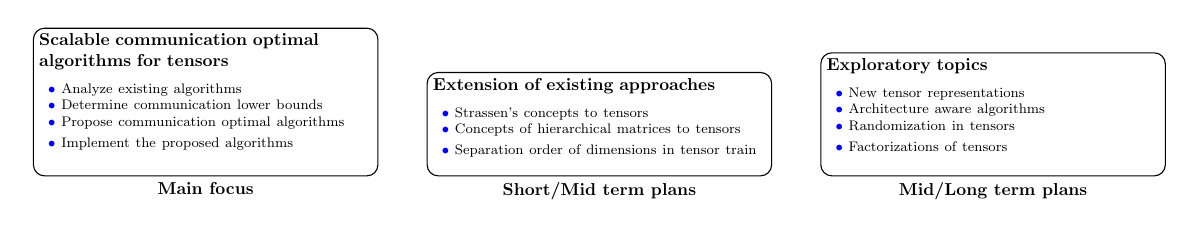
\begin{tikzpicture}[scale=0.625, every node/.style={transform shape}]
\tikzstyle{taskr}=[draw=black, rounded corners, minimum height=30mm, minimum width=70mm, fill=none, text=black]


%%\tikzstyle{taskcompute}=[draw=black, minimum height=16mm, minimum width=16mm, fill=none, text=black, below]


\node (mainfocus) at (0,0) [taskr, anchor=south] {};
\node at (mainfocus.south) [below] {\textbf{Main focus}};

\node [below, align=left, text width=70mm]at (mainfocus.north) {		\textbf{$\ $Scalable communication optimal\\ $\ $algorithms for tensors\medskip}\\{\footnotesize \mybullet Analyze existing algorithms\\ 
	\mybullet Determine communication lower bounds\\\mybullet Propose communication optimal algorithms\\\mybullet Implement the proposed algorithms}};


\node (shorttermfocus) at (8,0) [taskr, minimum height=21mm, anchor=south] {};
\node at (shorttermfocus.south) [below] {\textbf{Short/Mid term plans}};

\node [below, align=left, text width=70mm]at (shorttermfocus.north) {\textbf{$\ $Extension of existing approaches\medskip}\\\footnotesize \mybullet Strassen's concepts to tensors\\\mybullet Concepts of hierarchical matrices to tensors\\\mybullet Separation order of dimensions in tensor train};


\node (midtermfocus) at (16,0) [taskr, minimum height=25mm, anchor=south] {};
\node at (midtermfocus.south) [below] {\textbf{Mid/Long term plans}};

\node [below, align=left, text width=70mm]at (midtermfocus.north) {\textbf{$\ $Exploratory topics\medskip}\\\footnotesize \mybullet New tensor representations\\ \mybullet Architecture aware algorithms\\ \mybullet Randomization in tensors\\ \mybullet Factorizations of tensors};

\end{tikzpicture}

\end{frame}


%%%%\begin{frame}{Test}
%%%%\begin{tikzpicture}[scale=0.625, every node/.style={transform shape}]
%%%%\tikzstyle{taskr}=[draw=black, rounded corners, minimum height=30mm, minimum width=70mm, fill=none, text=black]
%%%%
%%%%
%%%%%%\tikzstyle{taskcompute}=[draw=black, minimum height=16mm, minimum width=16mm, fill=none, text=black, below]
%%%%
%%%%
%%%%\node (mainfocus) at (0,0) [taskr, anchor=south] {};
%%%%\node at (mainfocus.south) [below] {\textbf{Main Focus}};
%%%%
%%%%\node [below, align=left, text width=70mm]at (mainfocus.north) {		\textbf{$\ $Scalable communication optimal algorithms for tensors}\\{\footnotesize \mybullet Analyze existing algorithms\\ 
%%%%		\mybullet Determine communication lower bounds\\\mybullet Propose communication optimal algorithms\\\mybullet Implement the proposed algorithms}};
%%%%
%%%%
%%%%\node (shorttermfocus) at (8,0) [taskr, minimum height=15mm, anchor=south] {};
%%%%\node at (shorttermfocus.south) [below] {\textbf{Short term plans}};
%%%%
%%%%\node [below, align=left, text width=70mm]at (shorttermfocus.north) {\footnotesize \mybullet Extend Strassen's concepts to tensors\\\mybullet Extend hierarchical matrices to tensors\\\mybullet Separation order of dimensions in tensor train};
%%%%
%%%%
%%%%\node (midtermfocus) at (16,0) [taskr, minimum height=20mm, anchor=south] {};
%%%%\node at (midtermfocus.south) [below] {\textbf{Mid term plans}};
%%%%
%%%%\node [below, align=left, text width=70mm]at (midtermfocus.north) {\footnotesize \mybullet New tensor representations\\ \mybullet Architecture aware algorithms\\ \mybullet Randomization in tensors\\ \mybullet Factorizations of tensors};
%%%%
%%%%
%%%%%%		\textbf{Scalable communication optimal algorithms for tensors}\\{\footnotesize $\quad$Analyze existing algorithms\\ 
%%%%%%		$\quad$Determine communication lower bounds\\$\quad$Propose communication optimal algorithms\\$\quad$Implement the proposed algorithms}};
%%%%
%%%%
%%%%
%%%%%%		\\Determine communication lower bounds\\Propose communication optimal algorithms\\Implement the proposed algorithms}};
%%%%
%%%%%%		\node (textmainfocus) at (mainfocus.south) [below] {Scalable communication optimal algorithms for tensors};
%%%%%%%%%%		\textbf{}}
%%%%\end{tikzpicture}
%%%%\end{frame}






%%\section{Communication and its importance in HPC}


\section{Design of Scalable Communication Optimal Algorithms for Tensors (Main Focus)}
%%\begin{frame}
%%\frametitle{Table of Contents}
%%\tableofcontents[currentsection]
%%\end{frame}

\begin{frame}{Scalabale algorithms for popular tensor operations}
\begin{itemize}
\item Determine the communication lower bounds for tensor decompositions
\item Analyse the popular decomposition algorithms and communications performed by them
\item Propose new scalable communication optimal algorithms
\begin{itemize}
\item If possible design tiles/tasks based algorithms
\end{itemize}
\item Implement the proposed algorithms
\begin{itemize}
\item Handle performance issues for homogeneous systems
\begin{itemize}
\item Load balancing
\item Memory aware approaches
\item scheduling strategies
\end{itemize}
\end{itemize}
\item Same for manipulation operations of popular tensor representations
\item Extend implementation for heterogeneous systems (start with Nvidia GPUs based heterogeneous systems)
\item Create a tensor library
\end{itemize}
\end{frame}



%%\begin{frame}{Tensor Diagram Notations }
%%%%$Tensors are denoted by solid shapes aand number of lines coming out of the shapes denote the dimensions of the tensors.$
%%\\
%%\noindent For example,
%%\begin{center}
%%	\begin{tabular}{ccc}
%%		Dimension & Name &\\
%%		1 & Vector & \begin{tikzpicture}[scale=0.5, every node/.style={transform shape}]
%%		\tikzstyle{taskc}=[circle, draw=black, minimum size=3mm, fill=\tensorcolor]
%%		\node (t01) at (0,0) [taskc]{};
%%		\draw (t01) -- (1,0);
%%		\path (t01) -- (-1,0);
%%		\end{tikzpicture} \\
%%		2 & Matrix & \begin{tikzpicture}[scale=0.5, every node/.style={transform shape}]
%%		\tikzstyle{taskc}=[circle, draw=black, minimum size=3mm, fill=\tensorcolor]
%%		\node (t01) at (0,0) [taskc]{};
%%		\draw (t01) -- (1,0);
%%		\draw (t01) -- (-1,0);
%%		\end{tikzpicture} \\
%%		3 & $3$-dimensional tensor & \begin{tikzpicture}[scale=0.5, every node/.style={transform shape}]
%%		\tikzstyle{taskc}=[circle, draw=black, minimum size=3mm, fill=\tensorcolor]
%%		\node (t01) at (0,0) [taskc]{};
%%		\draw (t01) -- (1,0);
%%		\draw (t01) -- (-1,0);
%%		\draw (t01) -- (0,1);	
%%		%%	\draw[<->,thin] (2, -0.2) -- node[below]{$3$} (4, -0.2);
%%		\end{tikzpicture}\\
%%	\end{tabular}
%%\end{center}

%%Tensors are denoted by solid shapes and number of lines coming out of the shapes denote the dimensions of the tensors.

%%\begin{itemize}
%%	\item Connecting two lines implies summation over the connected dimensions
%%	\item Multiplication of matrices \begin{tikzpicture}[scale=0.5, every node/.style={transform shape}]
%%	\tikzstyle{taskc}=[circle, draw=black, minimum size=5mm, fill=\tensorcolor]
%%	\node (t01) at (0,0) [taskc]{A};
%%	%%	\node [below] at (t01.south) {A};
%%	\draw (t01) -- node[above]{j}(1,0);
%%	\draw (t01) -- node[above]{i}(-1,0);
%%	%%	\draw (t01) -- (0,1);	
%%	%%	\draw[<->,thin] (2, -0.2) -- node[below]{$3$} (4, -0.2);
%%	\end{tikzpicture} and
%%	\begin{tikzpicture}[scale=0.5, every node/.style={transform shape}]
%%	\tikzstyle{taskc}=[circle, draw=black, minimum size=5mm, fill=\tensorcolor]
%%	\node (t01) at (0,0) [taskc]{B};
%%	%%	\node [below] at (t01.south) {A};
%%	\draw (t01) -- node[above]{k}(1,0);
%%	\draw (t01) -- node[above]{j}(-1,0);
%%	%%	\draw (t01) -- (0,1);	
%%	%%	\draw[<->,thin] (2, -0.2) -- node[below]{$3$} (4, -0.2);
%%	\end{tikzpicture} is represented as 
%%	\begin{tikzpicture}[scale=0.5, every node/.style={transform shape}]
%%	\tikzstyle{taskc}=[circle, draw=black, minimum size=5mm, fill=\tensorcolor]
%%	\node (t01) at (0,0) [taskc]{C};
%%	%%	\node [below] at (t01.south) {A};
%%	\draw (t01) -- node[above]{k}(1,0);
%%	\draw (t01) -- node[above]{i}(-1,0);
%%	%%	\draw (t01) -- (0,1);	
%%	%%	\draw[<->,thin] (2, -0.2) -- node[below]{$3$} (4, -0.2);
%%	\end{tikzpicture}
%%	=
%%	\begin{tikzpicture}[scale=0.5, every node/.style={transform shape}]
%%	\tikzstyle{taskc}=[circle, draw=black, minimum size=5mm, fill=\tensorcolor]
%%	\node (t01) at (0,0) [taskc]{A};
%%	%%	\node [below] at (t01.south) {A};
%%	%%	\draw (t01) -- node[above]{j}(1,0);
%%	\draw (t01) -- node[above]{i}(-1,0);
%%	
%%	\node (t02) at (2,0) [taskc]{B};
%%	%%	\node [below] at (t01.south) {A};
%%	\draw (t02) -- node[above]{k}(3,0);
%%	\draw (t01) -- node[above]{j}(t02);
%%	%%	\draw (t01) -- (0,1);	
%%	%%	\draw[<->,thin] (2, -0.2) -- node[below]{$3$} (4, -0.2);
%%	\end{tikzpicture}
%%	%%	\vfill
%%	
%%\end{itemize}
%%\end{frame}



\begin{frame}{Popular tensor decompositions}

{\footnotesize\vspace*{-0.175cm}
\begin{block}{Tucker decomposition}
\begin{minipage}{0.325\linewidth}
\begin{center}
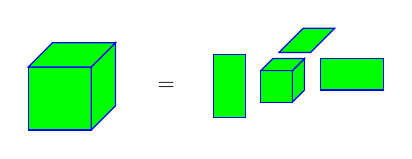
\begin{tikzpicture}[scale=0.2, every node/.style={transform shape}]
\pgfmathsetmacro{\cubex}{4}
\pgfmathsetmacro{\cubey}{4}
\pgfmathsetmacro{\cubez}{4}
\draw[blue,fill=pastelgreen] (-12,1,\cubez-2) -- ++(-\cubex,0,0) -- ++(0,-\cubey,0) -- ++(\cubex,0,0) -- cycle;
\draw[blue,fill=pastelgreen] (-12,1,\cubez-2) -- ++(0,0,-\cubez) -- ++(0,-\cubey,0) -- ++(0,0,\cubez) -- cycle;
\draw[blue,fill=pastelgreen] (-12,1,\cubez-2) -- ++(-\cubex,0,0) -- ++(0,0,-\cubez) -- ++(\cubex,0,0) -- cycle;
\node[draw=none, text=black, scale=4] at (-8,-1,0) {$=$};

\pgfmathsetmacro{\cubex}{2}
\pgfmathsetmacro{\cubey}{2}
\pgfmathsetmacro{\cubez}{2}
\draw[blue,fill=pastelgreen] (0,0,0) -- ++(-\cubex,0,0) -- ++(0,-\cubey,0) -- ++(\cubex,0,0) -- cycle;
\draw[blue,fill=pastelgreen] (0,0,0) -- ++(0,0,-\cubez) -- ++(0,-\cubey,0) -- ++(0,0,\cubez) -- cycle;
\draw[blue,fill=pastelgreen] (0,0,0) -- ++(-\cubex,0,0) -- ++(0,0,-\cubez) -- ++(\cubex,0,0) -- cycle;

\draw[blue,fill=pastelgreen] (-\cubex-1,1,0) -- ++(-\cubex,0,0) -- ++(0,-\cubey-2,0) -- ++(\cubex,0,0) -- cycle;
\draw[blue,fill=pastelgreen] (\cubex+2+1,0,-\cubey) -- ++(-\cubex-2,0,0) -- ++(0,-\cubey,0) -- ++(\cubex+2,0,0) -- cycle;

\draw[blue,fill=pastelgreen] (0,0,-\cubez-1) -- ++(-\cubex,0,0) -- ++(0,0,-\cubez-2) -- ++(\cubex,0,0) -- cycle;
\end{tikzpicture}
\end{center}
\end{minipage}
\begin{minipage}{0.665\linewidth}
\begin{itemize}
\item Determine communication lower bounds for this operation
\item Analyse communications performed by state of the art algorithms
\item Propose and implement new scalable communication algorithms
\end{itemize}
\end{minipage}
\end{block}\vspace*{-0.15cm}
\begin{block}{Canonical decomposition}
\begin{minipage}{0.325\linewidth}
\begin{center}
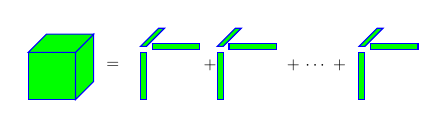
\begin{tikzpicture}[scale=0.15, every node/.style={transform shape}]
\pgfmathsetmacro{\cubex}{4}
\pgfmathsetmacro{\cubey}{4}
\pgfmathsetmacro{\cubez}{4}
\draw[blue,fill=pastelgreen] (0,0,0) -- ++(-\cubex,0,0) -- ++(0,-\cubey,0) -- ++(\cubex,0,0) -- cycle;
\draw[blue,fill=pastelgreen] (0,0,0) -- ++(0,0,-\cubez) -- ++(0,-\cubey,0) -- ++(0,0,\cubez) -- cycle;
\draw[blue,fill=pastelgreen] (0,0,0) -- ++(-\cubex,0,0) -- ++(0,0,-\cubez) -- ++(\cubex,0,0) -- cycle;

\node[draw=none, text=black, scale=4] at (2,-2.25,-3) {$=$};
\pgfmathsetmacro{\smallwidth}{0.5}
\draw[blue,fill=pastelgreen] (\cubex+2,0,0) -- ++(-\smallwidth,0,0) -- ++(0,-\cubey,0) -- ++(\smallwidth,0,0) -- cycle;
\draw[blue,fill=pastelgreen] (\cubex+2 +\cubex + 0.5,0.75,0) -- ++(-\cubex,0,0) -- ++(0,-\smallwidth,0) -- ++(\cubex,0,0) -- cycle;
\draw[blue,fill=pastelgreen] (\cubex+2,0.5,0) -- ++(-\smallwidth,0,0) -- ++(0,0,-\cubez) -- ++(\smallwidth,0,0) -- cycle;

\node[draw=none, text=black, scale=4] at (2+\cubex+4.25,-2.25,-3) {$+$};

\draw[blue,fill=pastelgreen] (\cubex+2.5 + \cubex+2,0,0) -- ++(-\smallwidth,0,0) -- ++(0,-\cubey,0) -- ++(\smallwidth,0,0) -- cycle;
\draw[blue,fill=pastelgreen] (\cubex+2.5+\cubex+2 +\cubex + 0.5,0.75,0) -- ++(-\cubex,0,0) -- ++(0,-\smallwidth,0) -- ++(\cubex,0,0) -- cycle;
\draw[blue,fill=pastelgreen] (\cubex+2.5+\cubex+2,0.5,0) -- ++(-\smallwidth,0,0) -- ++(0,0,-\cubez) -- ++(\smallwidth,0,0) -- cycle;

\node[draw=none, text=black, scale=4] at (2+\cubex+5 + \cubex+ 4.25, -2.25,-3) {$+$ $\cdots$ $+$};

\draw[blue,fill=pastelgreen] (12 + \cubex+2.5 + \cubex+2,0,0) -- ++(-\smallwidth,0,0) -- ++(0,-\cubey,0) -- ++(\smallwidth,0,0) -- cycle;
\draw[blue,fill=pastelgreen] (12+\cubex+2.5+\cubex+2 +\cubex + 0.5,0.75,0) -- ++(-\cubex,0,0) -- ++(0,-\smallwidth,0) -- ++(\cubex,0,0) -- cycle;
\draw[blue,fill=pastelgreen] (12 + \cubex+2.5+\cubex+2,0.5,0) -- ++(-\smallwidth,0,0) -- ++(0,0,-\cubez) -- ++(\smallwidth,0,0) -- cycle;

\end{tikzpicture}
\end{center}
\end{minipage}
\begin{minipage}{0.665\linewidth}
\begin{itemize}
\item No deterministic algorithm to find the decomposition
\item Analyse one iteration of the popular existing algorithms
%%			\item Matricized tensor times Khatri-Rao product (MTTKRP)  is the most time consuming operation
%%			\begin{itemize}
%%				\item MTTKRP: ({$\mathcal{X}$}, \{$A_1, \cdots ,A_{k-1}, A_{k+1},\cdots,A_d$\}) $\longrightarrow$ $A_k$
%%			\end{itemize}
%%			\item Determine communication lower bounds for MTTKRP operation

\item Propose and implement scalable algorithms for one iteration
\end{itemize}	
\end{minipage}
\end{block}\vspace*{-0.15cm}
\begin{block}{Tensor Train decomposition}
\begin{minipage}{0.325\linewidth}
\begin{center}
\begin{tikzpicture}[scale=0.25, every node/.style={transform shape}]

\node (t0) at (0,-2) [scale=4] {\tensor{A}};
\node [scale=4]at (2, -2) {$=$};
\path (5,-5) -- (0,0);
\end{tikzpicture}\hspace*{-0.25cm}
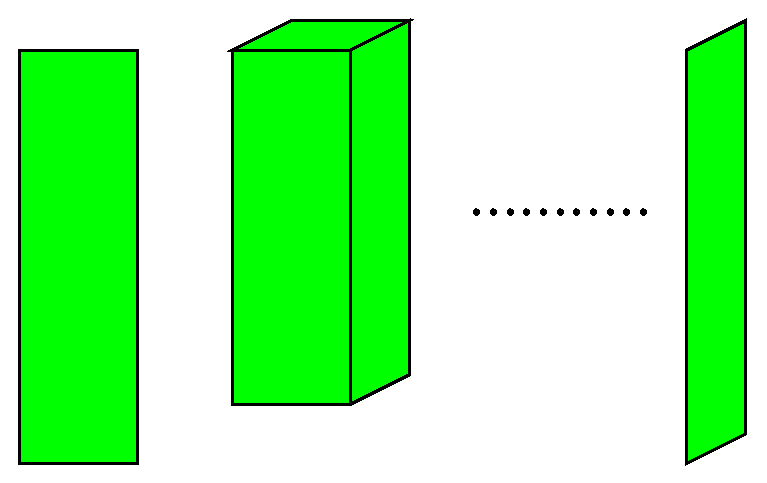
\includegraphics[scale=0.165]{./ttentry-simple.eps}
\end{center}
\end{minipage}
\begin{minipage}{0.665\linewidth}
\begin{itemize}
\item Determine communication lower bounds for this operation
\vfill
\item Analyse communication performed by popular algorithm
%%			: \textcolor{green}{Completed}
\vfill
\item Propose and implement new scalable communication algorithms
\end{itemize}
\end{minipage}
\end{block}
}
\end{frame}





\begin{frame}{Proving communication lower bounds for parallel computations}
\vspace*{-0.15cm}
{\footnotesize\begin{block}{How people did it for linear algebra operations?}
		\begin{itemize}
			\item People obtain results for matrix multiplication operations
			\item Same lower bounds apply to almost all direct linear linear algebra operations using reduction [Ballard et. al., 09]
			, for instance, bound for LU factorization\vspace*{-0.15cm}
			{\scriptsize\begin{align*}
				\begin{pmatrix}
				I &  & -B\\
				A & I &  &\\
				& & I
				\end{pmatrix}
				&=
				\begin{pmatrix}
				I & &\\
				A & I & \\
				&& I
				\end{pmatrix}
				\begin{pmatrix}
				I & & -B \\
				& I & AB\\
				& & I
				\end{pmatrix}
				\end{align*}}
		\end{itemize}
	\end{block}
	
	\vspace*{-0.15cm}{\footnotesize\begin{block}{Approach to compute lower bounds for tensor computations}
			Notation: Tensors are denoted by solid shapes and number of lines denote the dimensions of the tensors. Connecting two lines implies summation (or contraction) over the connected dimensions. 	
			\begin{itemize}
				\item Obtain bounds for basic tensor operations: Tensor times matrix (TTM), Multiple tensor times matrix (Multi-TTM), Tensor contraction
				
				
				%%		\includegraphics[scale=0.02]{./tmp/tensorBasicOperations.jpg}
				\vspace*{-0.25cm}\begin{center}
					%%	 \begin{tikzpicture}[scale=0.45, every node/.style={transform shape}]
					%%	\tikzstyle{taskc}=[circle, draw=black, minimum size=3mm, fill=\tensorcolor]
					%%	\node (t01) at (0,0) [taskc]{};
					%%	\draw (t01) -- (0.75,0);
					%%	\draw (t01) -- (-0.75,0);
					%%	\draw (t01) -- (0,0.75);
					%%	\node (t02) at (0,0.75) [taskc]{};
					%%	
					%%	\path (0,-0.75) -- (0,-0.75);
					%%	\end{tikzpicture} $\qquad$
					\begin{tikzpicture}[scale=0.45, every node/.style={transform shape}]
					\tikzstyle{taskc}=[circle, draw=black, minimum size=3mm, fill=\tensorcolor]
					\node (t01) at (0,0) [taskc]{};
					\draw (t01) -- (1.5,0);
					\draw (t01) -- (-0.75,0);
					\draw (t01) -- (0,0.75);
					\draw (t01) -- (0,-0.75);
					\node (t02) at (0.75,0) [taskc]{};
					
					\path (0, -0.95) -- (0, 0.95);
					
					\end{tikzpicture} $\qquad$
					\begin{tikzpicture}[scale=0.45, every node/.style={transform shape}]
					\tikzstyle{taskc}=[circle, draw=black, minimum size=3mm, fill=\tensorcolor]
					
					
					%%	\node (t01) at (0,-0.75) [taskc]{};
					%%	\node (t02) at (0.56,-0.56) [taskc]{};
					%%	\node (t03) at (0.56, 0.56) [taskc]{};
					%%	\node (t04) at (0,0.75) [taskc]{};
					%%	\node (t05) at (-0.56, 0.56) [taskc]{};
					%%	\node (t06) at (-0.56, -0.56) [taskc]{};
					%%	
					%%	
					%%	\draw (t01) -- (t04);
					%%	\draw (t02) -- (t05);
					%%	\draw (t03) -- (t06);
					
					\draw (-0.95, 0) -- (0.95, 0);
					\draw (0, -0.95) -- (0, 0.95);	
					
					\node (t01) at (0,-0.55) [taskc]{};
					\node (t02) at (0,0.55) [taskc]{};
					\node (t03) at (-0.55, 0) [taskc]{};
					\node (t04) at (0.55, 0) [taskc]{};
					
					
					\node (t00) at (0,0) [taskc]{};
					
					\path (0, -0.95) -- (0, 0.95);
					
					%%	\draw (t01) -- (0.75,0);
					%%	\draw (t01) -- (-0.75,0);
					%%	\draw (t01) -- (0,0.75);
					%%	\draw (t01) -- (0,-0.75);
					%%	\node (t02) at (0.75,0) [taskc]{};
					\end{tikzpicture} $\qquad$
					\begin{tikzpicture}[scale=0.45, every node/.style={transform shape}]
					\tikzstyle{taskc}=[circle, draw=black, minimum size=3mm, fill=\tensorcolor]
					\node (t01) at (0,0) [taskc]{};
					\draw (t01) -- (0.75,0);
					\draw (t01) -- (-0.75,0);
					\draw (t01) -- (0,0.75);
					\draw (t01) -- (0,-0.75);
					\draw (t01) -- (-0.56, -0.56);
					
					\node (t02) at (0.75,0) [taskc]{};
					\draw (t02) -- (0.75,0.75);
					\draw (t02) -- (0.75,-0.75);
					
					\path (0, -0.95) -- (0, 0.95);
					\end{tikzpicture}
				\end{center}
				\vspace*{-0.25cm}				
				\item Express decompositions and manipulations in terms of these basis operations
			\end{itemize}
	\end{block}}
}\end{frame}




\section{Extension of Existing Approaches/Algorithms (Short/Mid Term Research Plans)}
%%\begin{frame}
%%\frametitle{Research Project}
%%\tableofcontents[currentsection]
%%\end{frame}
%%\subsubsection{Tensor Contraction and Strassen's Matrix Multiplication}
%%\begin{frame}{Tensor Contraction \& Strassen's Matrix Multiplication}
%%content...
%%\end{frame}


\begin{frame}{Strassen's concepts to tensors}
\vspace*{-0.175cm}
{\footnotesize
\begin{block}{Matrix multiplication of $n\times n$ square matrices }
	\begin{itemize}
		\item Complexity of traditional matrix multiplication is $\mathcal{O}(n^3)$ 
		\item Strassen's matrix multiplication
		\begin{itemize}
			\item Expressed matrix multiplication as a tensor computation
			\item Canonical rank of the tensor determines the complexity of the computation
			\item Complexity is $\mathcal{O}(n^{2.81})$
		\end{itemize}
		\item Plan to extend Strassen's concepts to tensor contractions
	\end{itemize}
\end{block}}\vspace*{-0.15cm}
\begin{exampleblock}{Contraction of a 3-dimensional tensor with a matrix}{\scriptsize
	\begin{minipage}{0.5\linewidth}\vspace*{-0.05cm}
		\begin{algorithmic}
			\FOR{$i_1=1:n$}
			\FOR{$i_2=1:n$}
			\FOR{$i_3=1:n$}
			\FOR{$j_2=1:n$} 
			\STATE {$\tensor{G}(i_1,i_2,j_2) = \tensor{G}(i_1,i_2,j_2) + \tensor{A}(i_1,i_2,i_3)*B(i_3,j_2)$} 
			\ENDFOR
			\ENDFOR
			\ENDFOR
			\ENDFOR
		\end{algorithmic}
	\end{minipage}
	\begin{minipage}{0.45\linewidth}{\footnotesize
			\begin{itemize}
				\item Total $\mathcal{O}(n^{4})$ operations
				\item Apply Strassen's algorithm for each $i_1$, total $\mathcal{O}(n^{3.81})$ operations 
				\item Expressing as a canonical decomposition of $8\times8\times4$ tensor can further reduces the number of operations
			\end{itemize}
	}\end{minipage}
}\end{exampleblock}
\end{frame}


\begin{frame}{Hierarchical Matrix concepts to Tensors}
\begin{block}{Hierarchical Matrices}
	\begin{itemize}
		\item Data sparse approximation of non-sparse matrices
		\begin{center}
			
			\begin{tikzpicture}[scale=0.425, every node/.style={transform shape}]
			
			\tikzstyle{taskr}=[draw=black, minimum height=32mm, minimum width=32mm, fill=none, text=black]
			
			\node (t0) at (0,0) [taskr] {};
			\node [below,scale=1.5] at (t0.south) {Original Matrix};
			
			\end{tikzpicture}$\qquad\qquad$
			\begin{tikzpicture}[scale=0.425, every node/.style={transform shape}]
			
			\tikzstyle{taskr}=[draw=black, minimum height=32mm, minimum width=32mm, fill=none, text=black]
			
			\node (t0) at (0,0) [taskr] {};
			\node [below,scale=1.5] at (t0.south) {Step 1};
			
			\node (t00) at (0,0) [taskr, anchor=north east, minimum width=16mm, minimum height=16mm] {LR};
			\node (t00) at (0,0) [taskr, anchor=south west, minimum width=16mm, minimum height=16mm] {LR};
			
			\end{tikzpicture}$\qquad\qquad$
			\begin{tikzpicture}[scale=0.425, every node/.style={transform shape}]
			
			\tikzstyle{taskr}=[draw=black, minimum height=32mm, minimum width=32mm, fill=none, text=black]
			
			\node (t0) at (0,0) [taskr] {};
			\node [below,scale=1.5] at (t0.south) {Step 2};
			
			\node (t00) at (0,0) [taskr, anchor=north east, minimum width=16mm, minimum height=16mm] {LR};
			\node (t00) at (0,0) [taskr, anchor=south west, minimum width=16mm, minimum height=16mm] {LR};
			
			
			
			\node (t000) at (t0.west) [taskr, anchor=south west, minimum width=8mm, minimum height=8mm] {LR};
			\node (t001) at (t000.north east) [taskr, anchor=south west, minimum width=8mm, minimum height=8mm] {LR};
			
			\node (t000) at (t0.south) [taskr, anchor=south west, minimum width=8mm, minimum height=8mm] {LR};
			\node (t001) at (t000.north east) [taskr, anchor=south west, minimum width=8mm, minimum height=8mm] {LR};
			\end{tikzpicture}
		\end{center}
	\end{itemize}
	\noindent $LR$: low rank block
\end{block}

\begin{block}{Tensors}
	\begin{minipage}{0.565\linewidth}
		\begin{itemize}
			\item $f(i,j,k) = \frac{1}{|i-j|+|j-k|+|k-i|}$
			\item Value is small if difference of any pair is large
			\item Formalize and evaluate this approach for tensors
		\end{itemize}
	\end{minipage}
	\begin{minipage}{0.4\linewidth}
		\begin{center}
			\begin{tikzpicture}[scale=0.5, every node/.style={transform shape}]
			
			\def\xref{0.6}
			\def\yref{0.5}
			
			\draw (0,0) -- (2,0)--(2,2)--(0,2)--(0,0);
			\draw (2,0) -- (2+2*\xref, 2*\yref) -- (2+2*\xref, 2+2*\yref) -- (2,2) -- (2,0);
			\draw (0,2) -- (2,2) -- (2+2*\xref, 2+2*\yref) -- (2*\xref, 2+2*\yref) --(0,2);
			\node [below] at (1,0) {Original Tensor};
			\end{tikzpicture}$\qquad\qquad$
			\begin{tikzpicture}[scale=0.5, every node/.style={transform shape}]
			%%\draw[thin] (-2, 0) -- node[above,scale=0.85]{$A(0,0)$} (-1, 0) -- (-1,1) -- (-2,1) -- (-2,0) ;
			\draw (0,0) -- node [above] {LR}(1,0) -- (1,1) -- (0,1)--(0,0);
			\draw (1,0) -- node [above] {LR}(2,0) -- (2,1) -- (1,1)--(1,0);
			\draw [fill=green] (0,1) -- (1,1) -- (1,2) -- (0,2)--(0,1);
			\draw  (1,1) -- node [above] {LR}(2,1) -- (2,2) -- (1,2)--(1,1);
			
			\def\xref{0.6}
			\def\yref{0.5}
			
			\draw (2,0) -- (2+\xref, \yref) -- (2+\xref, \yref +1) -- (2,1) -- (2,0);
			\draw (2,1) -- (2+\xref, 1+\yref) -- (2+\xref, 2+\yref ) -- (2,2) -- (2,1);
			
			\draw [fill=green](2+\xref,0+\yref) -- (2+2*\xref, 2*\yref) -- (2+2*\xref, 2*\yref +1) -- (2+\xref,1+\yref) -- (2+\xref,\yref);
			\draw (2+\xref,1+\yref) -- node [above] {LR}(2+2*\xref, 1+2*\yref) -- (2+2*\xref, 2*\yref +2) -- (2+\xref,2+\yref) -- (2+\xref,1+\yref);
			
			
			\draw [fill=green] (0,2) --  (1,2) -- (1+\xref, 2+\yref) -- (\xref, 2+\yref) -- (0,2);
			\draw (1,2) -- (2,2) -- (2+\xref, 2+\yref) -- (1+\xref, 2+\yref) -- (1,2);
			\draw (0+\xref,2+\yref) -- node [sloped, above right,rotate=0] {LR} (1+\xref,2+\yref) -- (1+2*\xref, 2+2*\yref) -- (2*\xref, 2+2*\yref) -- (0+\xref,2+\yref);
			\draw (1+\xref,2+\yref) --  (2+\xref,2+\yref) -- (2+2*\xref, 2+2*\yref) -- (1+2*\xref, 2+2*\yref) -- (1+\xref,2+\yref);
			
			\node [below] at (1,0) {Step 1};
			
			\end{tikzpicture}
		\end{center}
	\end{minipage}
\end{block}
\end{frame}


\section{Exploratory Topics (Mid/Long Term Research Plans)}
%%\begin{frame}
%%\frametitle{Research Project}
%%\tableofcontents[currentsection]
%%\end{frame}

\begin{frame}{High Dimensional Tensor Representations and Randomization}
\begin{itemize}
\item Tensor Train is a popular representation to work with high dimensional tensors
\item Adding tensors and aplying an operator in this representation
\begin{minipage}{0.475\linewidth}
	\begin{center}
		\begin{tikzpicture}[scale=0.35, every node/.style={transform shape}]
		\tikzstyle{taskc}=[circle, draw=black, minimum size=5mm, fill=\tensorcolor]
		%%	\node (t01) at (0,0) [taskc]{};
		
		\draw (2,0) -- (-2,0);
		
		\foreach \x in {1, 0.5, 0, -0.5, -1}
		\draw (2*\x, 0) -- (2*\x,0.75);
		
		\foreach \x in {1, 0.5, 0, -0.5, -1}
		\node at (2*\x, 0) [taskc] {};
		
		\node [below,scale=1.5] at (0,-1) {rank=$r$};
		
		\node [scale=2] at (3.25, 0) {$+\ $};
		
		\path (0, 1.45) -- (0, -1.45);
		\end{tikzpicture}
		\begin{tikzpicture}[scale=0.35, every node/.style={transform shape}]
		\tikzstyle{taskc}=[circle, draw=black, minimum size=5mm, fill=\tensorcolor]
		%%	\node (t01) at (0,0) [taskc]{};
		
		\draw (2,0) -- (-2,0);
		
		\foreach \x in {1, 0.5, 0, -0.5, -1}
		\draw (2*\x, 0) -- (2*\x,0.75);
		
		\foreach \x in {1, 0.5, 0, -0.5, -1}
		\node at (2*\x, 0) [taskc] {};
		
		\node [below,scale=1.5] at (0,-1) {rank=$s$};
		
		\node [scale=2] at (3.25, 0) {$=\ $};
		\path (0, 1.45) -- (0, -1.45);
		\end{tikzpicture}
		\begin{tikzpicture}[scale=0.35, every node/.style={transform shape}]
		\tikzstyle{taskc}=[circle, draw=black, minimum size=5mm, fill=\tensorcolor]
		%%	\node (t01) at (0,0) [taskc]{};
		
		\draw (2,0) -- (-2,0);
		
		\foreach \x in {1, 0.5, 0, -0.5, -1}
		\draw (2*\x, 0) -- (2*\x,0.75);
		
		\foreach \x in {1, 0.5, 0, -0.5, -1}
		\node at (2*\x, 0) [taskc] {};
		
		\node [below,scale=1.5] at (0,-1) {rank=$r+s$};
		\path (0, 1.45) -- (0, -1.45);
		\end{tikzpicture}
	\end{center}
\end{minipage}$\quad$
\begin{minipage}{0.475\linewidth}
	%%	\item Applying an operator in this representation
	\begin{center}
		\begin{tikzpicture}[scale=0.35, every node/.style={transform shape}]
		\tikzstyle{taskc}=[circle, draw=black, minimum size=5mm, fill=\tensorcolor]
		%%	\node (t01) at (0,0) [taskc]{};
		
		\draw (2,0) -- (-2,0);
		
		\foreach \x in {1, 0.5, 0, -0.5, -1}
		\draw (2*\x, 0) -- (2*\x,0.75);
		
		\foreach \x in {1, 0.5, 0, -0.5, -1}
		\node at (2*\x, 0) [taskc] {};
		
		\node [below,scale=1.5] at (0,-1) {rank=$r$};
		
		\node [scale=2] at (3.25, 0) {$\ $};
		\path (0, 1.45) -- (0, -1.45);
		\end{tikzpicture}
		\begin{tikzpicture}[scale=0.35, every node/.style={transform shape}]
		\tikzstyle{taskc}=[circle, draw=black, minimum size=5mm, fill=\tensorcolor]
		%%	\node (t01) at (0,0) [taskc]{};
		
		\draw (2,0) -- (-2,0);
		
		\foreach \x in {1, 0.5, 0, -0.5, -1}
		\draw (2*\x, 0) -- (2*\x,0.75);
		
		\foreach \x in {1, 0.5, 0, -0.5, -1}
		\draw (2*\x, 0) -- (2*\x,-0.75);
		
		\foreach \x in {1, 0.5, 0, -0.5, -1}
		\node at (2*\x, 0) [taskc] {};
		
		\node [below,scale=1.5] at (0,-1) {rank=$s$};
		
		\node [scale=2] at (3.25, 0) {$=\ $};
		\path (0, 1.45) -- (0, -1.45);
		\end{tikzpicture}
		\begin{tikzpicture}[scale=0.35, every node/.style={transform shape}]
		\tikzstyle{taskc}=[circle, draw=black, minimum size=5mm, fill=\tensorcolor]
		%%	\node (t01) at (0,0) [taskc]{};
		
		\draw (2,0) -- (-2,0);
		
		\foreach \x in {1, 0.5, 0, -0.5, -1}
		\draw (2*\x, 0) -- (2*\x,0.75);
		
		\foreach \x in {1, 0.5, 0, -0.5, -1}
		\node at (2*\x, 0) [taskc] {};
		
		\node [below,scale=1.5] at (0,-1) {rank=$r*s$};
		\path (0, 1.45) -- (0, -1.45);
		\end{tikzpicture}
	\end{center}
\end{minipage}

\item Requires a truncation  process which iterates over cores one by one 
\item This representation is not much suited to work in parallel 
\end{itemize}

\begin{block}{\footnotesize New tensor representations}
\begin{itemize}
	\item Look at new representations in tree format -- suitable for parallelization
	%%	\vfill
	\begin{center}
		\begin{tikzpicture}[scale=0.275, every node/.style={transform shape}]
		\tikzstyle{taskc}=[circle, draw=black, minimum size=5mm, fill=\tensorcolor]
		
		\node (t) at (0,0) [taskc]{};
		\node (t0) at (-1,-1) [taskc]{};
		\node (t00) at (-2,-2) [taskc]{};
		\node (t01) at (-0.5,-2) [taskc]{};
		\node (t000) at (-3,-3) [taskc]{};
		\node (t001) at (-1.8,-3) [taskc]{};
		\node (t010) at (-1,-3) [taskc]{};
		\node (t011) at (-0.285,-3) [taskc]{};
		
		\draw (t) -- (t0);
		\draw (t0) -- (t00);
		\draw (t0) -- (t01);
		\draw (t00) -- (t000);
		\draw (t00) -- (t001);
		\draw (t01) -- (t010);
		\draw (t01) -- (t011);
		
		
		\node (t1) at (1,-1) [taskc]{};
		\node (t10) at (0.5,-2) [taskc]{};
		\node (t11) at (2,-2) [taskc]{};
		\node (t100) at (0.285,-3) [taskc]{};
		\node (t101) at (1,-3) [taskc]{};
		\node (t110) at (1.8,-3) [taskc]{};
		\node (t111) at (3,-3) [taskc]{};
		
		\draw (t) -- (t1);
		\draw (t1) -- (t10);
		\draw (t1) -- (t11);
		\draw (t10) -- (t100);
		\draw (t10) -- (t101);
		\draw (t11) -- (t110);
		\draw (t11) -- (t111);
		
		\node [scale=2] at (4.5,-2) {or};
		\end{tikzpicture} $\qquad$
		\begin{tikzpicture}[scale=0.275, every node/.style={transform shape}]
		\tikzstyle{taskc}=[circle, draw=black, minimum size=5mm, fill=\tensorcolor]
		
		\node (t) at (0,0) [taskc]{};
		\node (t0) at (-1,-1) [taskc]{};
		\node (t00) at (-2,-2) [taskc]{};
		\node (t01) at (-0.5,-2) [taskc]{};
		\node (t000) at (-3,-3) [taskc]{};
		\node (t001) at (-1.8,-3) [taskc]{};
		\node (t010) at (-1,-3) [taskc]{};
		\node (t011) at (-0.285,-3) [taskc]{};
		
		\draw (t) -- (t0);
		\draw (t0) -- (t00);
		\draw (t0) -- (t01);
		\draw (t00) -- (t000);
		\draw (t00) -- (t001);
		\draw (t01) -- (t010);
		\draw (t01) -- (t011);
		
		
		\node (t1) at (1,-1) [taskc]{};
		\node (t10) at (0.5,-2) [taskc]{};
		\node (t11) at (2,-2) [taskc]{};
		\node (t100) at (0.285,-3) [taskc]{};
		\node (t101) at (1,-3) [taskc]{};
		\node (t110) at (1.8,-3) [taskc]{};
		\node (t111) at (3,-3) [taskc]{};
		
		\draw (t) -- (t1);
		\draw (t1) -- (t10);
		\draw (t1) -- (t11);
		\draw (t10) -- (t100);
		\draw (t10) -- (t101);
		\draw (t11) -- (t110);
		\draw (t11) -- (t111);
		
		%%		\draw [thick,green] (t0) -- (t1);
		%%		\draw [thick,green] (t00) -- (t01);
		%%		\draw [thick,green] (t000) -- (t001);
		%%		\draw [thick,green] (t010) -- (t011);
		%%		\draw [thick,green] (t10) -- (t11);
		%%		\draw [thick,green] (t100) -- (t101);
		%%		\draw [thick,green] (t110) -- (t111);
		
		\draw [thick,green] (t01) -- (t10);
		\end{tikzpicture} 
		%%			\includegraphics[scale=0.02]{./tmp/newTensorRepresenattion.jpg}
	\end{center}
	\begin{itemize}
		\item Data will be stored at the leaf nodes
%%		\item Interal nodes will help to manipulate tensors in parallel
	\end{itemize}
	%%	\vfill
	%%	\item Some tensor representations exhibit tree structure
	%%	\begin{itemize}
	%%		\item Mainly designed to reduce storage or model long range interactions
	%%		\item Not suitable to work with them in parallel
	%%	\end{itemize}
\end{itemize}
\end{block}
\begin{itemize}
	\item Apply randomization to tensor operations
\end{itemize}
\end{frame}


\begin{frame}{Architecture Aware Algorithms}
\begin{center}
	\begin{minipage}{0.45\columnwidth}
			\includegraphics[scale=0.25]{./VoltaTensorCore.png}
	\end{minipage}
	\begin{minipage}{0.45\columnwidth}
		\includegraphics[scale=0.25]{./A100_TensorCore_FP64.jpg}
	\end{minipage}
\end{center}
\begin{itemize}
	\item Recent Nvidia GPUs have tensor cores to accelerate AI computations
	\item Most linear algebra computations do not take advantages of these units
	\item Design algorithms which take architecture details into account
\end{itemize}
Fig source: \url{www.nvidia.com}
\end{frame}


%%\begin{frame}{Randomization in Tensor Computations}
%%\begin{itemize}
%%\item Randomized SVD and UTV factorization are now well established
%%\vfill
%%\item Apply randomization to tensors
%%\vfill
%%\item Perform factorizations of tensors
%%\begin{itemize}
%%\item For example: QR like factorization of a tensor
%%\end{itemize}
%%\begin{center}
%%\begin{tikzpicture}[scale=0.5, every node/.style={transform shape}]
%%\tikzstyle{taske}=[ellipse, draw=black, minimum width=25mm, minimum height=8mm, fill=\tensorcolor]
%%\node (t0) at (0,0) [taske] {};
%%
%%\foreach \x in {1, 0.75, 0.5, 0.25, 0, -0.25, -0.5, -0.75, -1}
%%\draw (\x, 0.75) -- (\x, 0);
%%
%%%%	\foreach \y/\l in { 0/{0.4/0, 0.3/0.4, 0.7/0.7}, 
%%%%		0.5/{0.3/0, 0.4/0.3, 0.3/0.7},
%%%%		1.25/{0.5/0, 0.3/0.5, 1.2/0.8, 1.5/2.0},
%%%%		1.75/{0.8/0, 0.4/0.8, 0.7/1.2, 0.5/1.9},
%%%%		2.25/{0.6/0, 0.4/0.6, 1.1/1.0, 1.0/2.1},
%%%%	} {
%%%%		\foreach \w/\x in \l
%%%%		\node at (\x, \y)[task, minimum width=\w cm, fill=white] {};
%%%%	}
%%
%%
%%\node (t0) at (0,0) [taske] {};
%%\end{tikzpicture}$\qquad$
%%\begin{tikzpicture}[scale=0.5, every node/.style={transform shape}]
%%\tikzstyle{taskc}=[circle, draw=black, minimum size=5mm, fill=\tensorcolor]
%%%%	\node (t01) at (0,0) [taskc]{};
%%
%%
%%
%%\draw (4,0) -- (-4,0);
%%
%%\foreach \x in {1, 0.75, 0.5, 0.25, 0, -0.25, -0.5, -0.75, -1}
%%\draw (4*\x, 0) -- (4*\x,0.75);
%%
%%\foreach \x in {1, 0.75, 0.5, 0.25, 0, -0.25, -0.5, -0.75, -1}
%%\node at (4*\x, 0) [taskc] {};
%%
%%\end{tikzpicture}
%%\end{center}
%%\end{itemize}
%%\end{frame}

\begin{frame}{Integration in the LIP/LaBRI laboratory}
%%\vspace*{-0.175cm}

{\footnotesize
\vspace*{0.15cm}
	%%\vspace*{-0.1cm}
	\begin{tikzpicture}[scale=0.625, every node/.style={transform shape}]
	\tikzstyle{taskr}=[draw=black, rounded corners, minimum height=30mm, minimum width=70mm, fill=none, text=black]
	
	
	%%\tikzstyle{taskcompute}=[draw=black, minimum height=16mm, minimum width=16mm, fill=none, text=black, below]
	
	
	\node (mainfocus) at (0,0) [taskr, minimum height=21mm, anchor=south] {};
	\node at (mainfocus.south) [below] {\textbf{Main focus}};
	
	\node [below, align=left, text width=70mm]at (mainfocus.north) {		\textbf{$\ $Communication optimal tensor algorithms\smallskip}\\{\footnotesize \mybullet Analyze existing algorithms\\ 
			\mybullet Determine communication lower bounds\\\mybullet Propose communication optimal algorithms\\\mybullet Implement the proposed algorithms}};
	
	
	\node (shorttermfocus) at (8,0) [taskr, minimum height=21mm, anchor=south] {};
	\node at (shorttermfocus.south) [below] {\textbf{Short/Mid term plans}};
	
	\node [below, align=left, text width=70mm]at (shorttermfocus.north) {\textbf{$\ $Extension of existing approaches\smallskip}\\\footnotesize \mybullet Strassen's concepts to tensors\\\mybullet Concepts of hierarchical matrices to tensors\\\mybullet Separation order of dimensions in tensor train};
	
	
	\node (midtermfocus) at (16,0) [taskr, minimum height=21mm, anchor=south] {};
	\node at (midtermfocus.south) [below] {\textbf{Mid/Long term plans}};
	
	\node [below, align=left, text width=70mm]at (midtermfocus.north) {\textbf{$\ $Exploratory topics\smallskip}\\\footnotesize \mybullet New tensor representations\\ \mybullet Architecture aware algorithms\\ \mybullet Randomization in tensors\\ \mybullet Factorizations of tensors};
	
	
	
%%%%	\tikzstyle{taske}=[ellipse, draw=black, minimum width=65mm, minimum height=30mm, fill=none]
%%%%	
%%%%	\node (expertise) at (10,4.75) [taske] {};
%%%%	\node at (expertise.south) [below] {\textbf{Expertise of the team}};
%%%%	\node [text width=56mm] at (expertise.mid) {\footnotesize \mybullet Parallel algorithms\\
%%%%		\mybullet Scheduling strategies\\
%%%%		\mybullet Memory aware algorithms\\
%%%%		\mybullet Sparse tensor computations\\
%%%%		\mybullet Low rank compression algorithms};
%%%%	
%%%%	
%%%%	\tikzstyle{taskt}=[ellipse, draw=black, minimum width=87.5mm, minimum height=15mm, fill=none]
%%%%	\node (team) at (1,5) [taskt] {};
%%%%	\node at (team.south) [below] {\textbf{Team}};
%%%%	\node [text width=70mm] at (team.mid) {Anne Benoit,
%%%%		Loris Marchal, 
%%%%		Gregoire Pichon,\\
%%%%		Yves Robert,
%%%%		Bora Ucar, and
%%%%		Frederic Vivien
%%%%	};
	
	
	
	%%	\node (bora) at (-1,5) [taske] {\textbf{Bora Ucar}};
	%%	\node [above, align=left, text width=35mm]at (bora.north) {Expert in sparse tensor computations};
	%%	
	%%	%%\draw [->] (bora) -- (mainfocus);
	%%	%%\draw [->] (bora) -- (shorttermfocus);
	%%	%%\draw [->] (bora) -- (midtermfocus);
	%%	
	%%	
	%%	\node (loris) at (4,5) [taske] {\textbf{$\ $Loris Marchal$\ $}};
	%%	\node [above, align=left, text width=42mm]at (loris.north) {Expert in communication and memory aware algorithms};
	%%	
	%%	%%\draw [->] (loris) -- (mainfocus);
	%%	%%\draw [->] (loris) -- (shorttermfocus);
	%%	%%\draw [->] (loris) -- (midtermfocus);
	%%	
	%%	
	%%	\node (others) at (11.8, 5) [taske, text width=40mm] {\textbf{Anne Benoit, Yves Robert and Frederic Vivien}};
	%%	\node [above, align=left, text width=60mm]at (others.north) {Expert in parallel algorithms and scheduling strategies};
	%%	
	%%	%%\draw [->] (others) -- (mainfocus);
	%%	%%\draw [->] (others) -- (shorttermfocus);
	%%	%%\draw [->] (others) -- (midtermfocus);
	%%	
	%%	
	%%	\node (gregoire) at (18, 5) [taske] {\textbf{Gregoire Pichon}};
	%%	\node [above, align=left, text width=40mm]at (gregoire.north) {Expert in low rank compression algorithms};
	%%	
	%%	%%\draw [->] (gregoire) -- (mainfocus);
	%%	%%\draw [->] (gregoire) -- (shorttermfocus);
	%%	%%\draw [->] (gregoire) -- (midtermfocus);
	
	\end{tikzpicture}
	
\vspace*{-0.15cm}
\begin{columns}{\scriptsize
		\begin{column}{0.485\linewidth}
			\begin{block}{\scriptsize ROMA team (LIP laboratory)}
				\begin{itemize}
					\item \emph{Bora Ucar}: design of tensor compression and manipulation algorithms
					\item \emph{Gregoire Pichon}: low-rank based algorithms
					\item  \emph{Anne Benoit, Loris Marchal, Yves Robert and Frederic Vivien}: scalability and scheduling aspects in the long term
				\end{itemize}
			\end{block}
		\end{column}
		\begin{column}{0.485\linewidth}		
			\begin{block}{\scriptsize SATANAS team (LaBRI laboratory)}
				\begin{itemize}
					\item \emph{Olivier Beaumont} and \emph{Lionel Eyraud-Dubois}: tensor train based neural network models
					\item \emph{Mathieu Faverge}: low-rank based methods
					\item  \emph{Abdou Guermouche, Samuel Thibault}: exploitation of maximum potential of HPC systems in the long term
				\end{itemize}
			\end{block}
		\end{column}
}\end{columns}
	
	\begin{block}{Bringing additional skills in the team}
		\begin{itemize}
			\item High dimensional dense tensor computations, use of tensors in molecular simulations
			\item Communication lower bounds for linear algebra computations
			\item Scalable approaches for large HPC systems
%%			\item Use of tensors in quantum and molecular simulations 
			%%		\item Designing strategies to work with high dimensional tensor computations
			%%		\item Determining communication lower bounds for linear algebra computations
			%%		\item Designing scalable approaches for large HPC systems
			%%		\item Familiar with molecular and quantum simulations and how tensors are used in these domains 
		\end{itemize}
	\end{block}
	
	
	
	%%\begin{itemize}
	%%	\item Design and implementation of scalable tensor algorithms (\textbf{Bora Ucar})
	%%%%	Expert in sparse tensor computations. Work with him on the design and implementation of scalable algorithms 
	%%	\item Memory aware algorithms for tensors (\textbf{Loris Marchal})
	%%%%	Expert in the design of memory and communication oriented algorithms. Work with him on extending the roofline model with dependencies and memory aware algorithms to schedule tasks on HPC platforms
	%%	\item Parallel algorithms and scheduling strategies for tasks of tensor operations on homogeneous/heterogeneous systems (\textbf{Anne Benoit}, \textbf{Yves Robert} and \textbf{Frederic Vivien})
	%%%%	Experts in designing parallel algorithms and scheduling strategies. Work with them on the design of scalable parallel algorithms and scheduling strategies for homogeneous/heterogeneous systems
	%%	\item Extension of hierarchical matrices to tensors (\textbf{Gregoire Pichon})
	%%%%	 Works on low rank compression of matrices. Work with him on extending the concept of hierarchical matrices to tensors
	%%\end{itemize}
}
\end{frame}

%%\begin{frame}
%%\Huge{\centerline{Thank You!}}
%%\end{frame}





\end{document} 